\documentclass{article}
\usepackage[utf8]{inputenc}
\usepackage{amsmath}
\usepackage{amssymb}
\usepackage{amsfonts}
\usepackage{bm}
\usepackage{graphicx}
\usepackage{caption}
\usepackage{subcaption}
\usepackage{authblk}
\usepackage{soul}
\usepackage{natbib}
\usepackage{authblk}
\bibliographystyle{custom_abbrvnat}%Import the bibliography file
\setcitestyle{authoryear,open={(},close={)}} 
\usepackage[letterpaper,top=2cm,bottom=2cm,left=3cm,right=3cm,marginparwidth=1.75cm]{geometry}
\usepackage[colorlinks=true, allcolors=blue]{hyperref}

\graphicspath{{\subfix{images/}}}

\title{Post-processing East African rainfall forecasts using a generative machine learning model}

\author[1,2]{Bobby Antonio}
\author[1]{Andrew McRae}
\author[3]{Dave MacLeod}
\author[1]{Fenwick Cooper}
\author[4]{John Marsham}
\author[5]{Laurence Aitchison}
\author[1]{Tim Palmer}
\author[2]{Peter Watson}


\affil[1]{Department of Physics, University of Oxford, Oxford, UK}
\affil[2]{School of Geographical Sciences, University of Bristol, Bristol, UK}
\affil[3]{School of Earth and Environment Sciences, University of Cardiff, Cardiff, UK}
\affil[4]{School of Earth and Environment, University of Leeds, Leeds,  UK}
\affil[5]{Machine Learning and Computational Neuroscience Unit, University of Bristol, Bristol, UK}









\begin{document}

\maketitle

\begin{abstract}
    Existing weather models are known to have poor skill at forecasting rainfall over East Africa, where there are regular threats of drought and floods presenting significant risks to people's lives and livelihoods. Improved precipitation forecasts could help mitigate the effects of these extreme weather events, as well as providing significant financial benefits to the region. Building on work that successfully applied a state-of-the-art machine learning method (a conditional Generative Adversarial Network, cGAN) to postprocess precipitation forecasts in the UK, we present a novel way to improve precipitation forecasts in East Africa. We address the challenge of realistically representing tropical rainfall in this region, where convection is dominant, which is poorly simulated in conventional global forecast models. We use a cGAN to postprocess short range hourly forecasts made by the European Centre for Medium-Range Weather Forecasts Integrated Forecast System at 6-18h lead times. Our forecasts have $0.1^{\circ}$ resolution. We investigate how well this method can correct biases, create samples of rainfall with realistic spatial structure and produce reliable probability distributions. The cGAN predictions and original forecast are also further postprocessed using a novel neighbourhood version of quantile mapping, in order to leverage the strengths of conventional postprocessing methods and provide a strong baseline to compare against. Our results indicate that the cGAN significantly improves the diurnal cycle of the IFS, and improves on metrics such as mean bias, and Fractions Skill Score up to high ($99.9^{\text{th}}$ percentile) rainfall values. However the quantile-mapped IFS achieves slightly higher Equitable Threat Score values at the grid scale. The cGAN ensemble exhibits a mixture of behaviours at different rainfall scales, with under-dispersion at low rainfall values and over-dispersion at high rainfall values. Overall our results demonstrate how the strengths of machine learning and conventional postprocessing methods can be combined, and illuminate where the benefits of machine learning for postprocessing lie. 
\end{abstract}

\section{Introduction}


East Africa experiences both severe droughts that cause famine \citep{gebremeskel_haile_droughts_2019} and extreme rainfall that significantly impacts the lives and livelihoods of those living in the region~\citep{kilavi_extreme_2018,wainwright_extreme_2021}. For example, flooding of the Shabelle river in Somalia in March 2023 affected an estimated 460,000 people~\citep{floodlist_somalia_2023}, and an estimated 3000-5000 people die on Lake Victoria every year as a result of storms that capsize boats~\citep{watkiss_socio-economic_2020}. 

More accurate forecasts are crucial for improving early earning systems and enabling schemes such as Forecast-based Financing to deliver aid and assistance to those affected~\citep{wilkinson_forecasting_2018}. Accurate rainfall forecasts are therefore crucial for improving attempts at mitigating the effects of these events, through enabling more accurate early warning systems, better disaster response, and agricultural planning. A recent study as part of the WISER project estimated that their work improving early warning systems brought benefits of £3m/yr due to early warning systems on the coast alone, plus additional intangible improvements to the well-being and safety of people living in the area~\citep{watkiss_socio-economic_2021}. Heavy rainfall advisories in Kenya have been demonstrated to be effective at predicting impactful rainfall events, especially over recent years, although there is still a need for increased resolution in the forecasts in order to better enable initiatives such as Forecast-based Financing~\citep{macleod_are_2021}.


Conventional forecast products that use convection parameterization have been demonstrated to capture the approximate relationship between rainfall variation in the East African tropics and drivers such as the Madden-Julian oscillations and Indian Ocean sea surface temperature. However, they tend to predict too many low intensity rainfall events and perform poorly at predicting heavy rainfall~\citep{woodhams_what_2018, chamberlain_forecasting_2014, vogel_skill_2018, walker_skill_2019, bechtold_representing_2014, haiden_intercomparison_2012}. Additionally, these models tend to do better at forecasting precipitation at longer than daily timescales, but do not model diurnal cycle of rainfall well~\citep{kim_tropical_2013, macleod_drivers_2021, bechtold_simulation_2004}, which is likely because of the convective parameterisation schemes used in the models~\citep{vogel_skill_2018, marsham_role_2013, bechtold_representing_2014}. 

In recent years, it has become computationally feasible to run `convection permitting' (CP) models at higher resolutions ($\sim4\text{km}$) for which the model can better capture convection processes without using a parameterization scheme. Several studies have investigated how well these CP models correct precipitation bias in East Africa~\citep{finney_implications_2019, cafaro_convection-permitting_2021, woodhams_what_2018, chamberlain_forecasting_2014, kendon_enhanced_2019, senior_convection-permitting_2021}; these studies have found that CP models tend to improve the overall rainfall distribution (at both high and low rainfall). They also tend to produce a more realistic rainfall frequency, as well as making the diurnal cycle more in line with observations. However, the rainfall distribution is not uniformly improved over the region~\citep{senior_convection-permitting_2021}, and many of these works demonstrate a tendency to over-predict rainfall. Some biases also still remain in diurnal cycle and intensity over the Lake Victoria region, and the models do not capture some of the nighttime peaks in areas such as South Sudan~\citep{finney_implications_2019, chamberlain_forecasting_2014}. 


% Existing numerical weather prediction (NWP) forecast products tend to struggle in tropical regions, particularly in capturing the intensity and diurnal cycle of precipitation, associated with the large role of convective rainfall in these regions, which is not well represented by convection parameterisation schemes used in existing global forecast models ~\citep{haiden_intercomparison_2012, vogel_skill_2018, woodhams_what_2018}. Convection-permitting models have demonstrated improved abilities at capturing the timing and intensity of rainfall~\citep{finney_implications_2019, woodhams_what_2018}, although there still appears to be a tendency for these models to over-predict rainfall in this region, and they are computationally expensive to run.

% Recent investigations into model performance also advocate that postprocessing may be required to improve skill in this region~\citep{vogel_skill_2018}.

At the same time machine learning models have improved dramatically over the last decade at a range of tasks, including generating realistic images~\citep{karras_style-based_2019}. This has inspired several attempts to create weather predictions from large amounts of historical data~\citep{nguyen_climax_2023, bi_pangu-weather_2022,ravuri_skilful_2021, zhang_skilful_2023,lam_graphcast_2022} and using machine learning for bias correction~\citep{rasp_neural_2018,ben-bouallegue_improving_2023}.

One of the most widely used machine learning models that can learn to sample realistic images from a target distribution is a Generative Adversarial Network or GAN~\citep{goodfellow_generative_2014}. Several works have demonstrated the effectiveness of GANs in a range of tasks; in \cite{leinonen_stochastic_2020} a GAN was trained to downscale low resolution observations~\citep{leinonen_stochastic_2020}.~\cite{harris_generative_2022} and~\cite{price_increasing_2022} then applied the same approach to the problem of downscaling coarse resolution forecasts towards radar observations. There are several works that have use GANs to postprocess precipitation forecasts: e.g.~\cite{duncan_generative_2022} have used a GAN to post-process the output of a machine learning model, and~\cite{jeong_correcting_2023} used a cyclical GAN to perform corrections of precipitation forecasts over South Korea. In addition to these approaches, other deep learning approaches have recently been successfully applied to post-processing climate and weather models, such as diffusion models~\citep{li_seeds_2023, addison_machine_2022, leinonen_latent_2023} and transformer models~\citep{ben-bouallegue_improving_2023}, and training neural networks using the energy score~\cite{pacchiardi_probabilistic_2021}.


However, only a small amount of effort has been applied to developing these techniques in tropical regions, such as regions in Africa, for which the need for improved forecasting is often greater, and which historically have not seen the same forecast skill improvements as mid-latitude areas like Europe and North America~\citep{youds_gcrf_2021}, and so we may be lacking a full view of the strengths of different models.

This raises the question; can we leverage recent advances in machine learning to improve forecasts in tropical regions such as East Africa? In this work we investigate this question by training a Generative Adversarial Network to postprocess short range NWP rainfall forecasts in East Africa at lead times of 6-18h, to test whether this can provide an effective means of correcting existing forecasts. We use forecasts from the state-of-the-art European Centre for Medium-Range Weather Forecasts (ECMWF) Integrated Forecast System (IFS) as the NWP product. In contrast to previous work on ML-based forecasting, we consider the challenging problem of forecasting rainfall in a tropical region, and evaluate whether a GAN is able to learn the properties of rainfall in a region where convection is dominant. We also combine the ML with a conventional postprocessing technique (quantile mapping), in order to leverage the strengths of both methods. We compare against ECMWF IFS forecasts, with quantile mapping also applied - this gives a baseline that is stronger than unmodified forecasts as commonly used in previous work on ML-based forecasting, giving a stronger test of whether ML can improve upon the state-of-the-art. 

This paper is structured as follows ... 


% \subsection{Statistical Post-processing}

% Statistical postprocessing techniques cover a wide spectrum, from simple methods such as subtracting the mean bias, to complex statistical and machine learning approaches (see~\cite{vannitsem_statistical_2021} for a comprehensive overview). 


% In this work we are concerned with producing short term precipitation forecasts that will be useful in applications such as flood modelling, and which achieve the highest resolution possible. For this reason we are particularly interested in statistical postprocessing techniques that can produce spatially realistic predictions, and that can produce an ensemble from a single deterministic forecast (since deterministic forecasts tend to be higher resolution than ensemble forecasts). Therefore previous approaches that predict the parameters of a known output probability distribution at each grid cell, such as~\citep{rasp_neural_2018}, or those that use deterministic models to correct forecasts~\citep{gronquist_deep_2021, han_deep_2021, horat_deep_2023} are not appropriate.

% One of the most widely used machine learning models that can learn to sample realistic images from a target distribution is a Generative Adversarial Network or GAN~\citep{goodfellow_generative_2014}. Several works have demonstrated the effectiveness of GANs in a range of tasks; in \cite{leinonen_stochastic_2020} a GAN was trained to downscale low resolution observations~\citep{leinonen_stochastic_2020}.~\cite{harris_generative_2022} and~\cite{price_increasing_2022} then applied the same approach to the problem of downscaling coarse resolution forecasts towards radar observations. There are several works that have use GANs to postprocess precipitation forecasts: e.g.~\cite{duncan_generative_2022} have used a GAN to post-process the output of a machine learning model, and~\cite{jeong_correcting_2023} used a cyclical GAN to perform corrections of precipitation forecasts over South Korea.

% Aside from GANs, other deep learning approaches that have recently been successfully applied to downscaling forecasts are diffusion models~\citep{li_seeds_2023, addison_machine_2022, leinonen_latent_2023} and transformer models~\citep{ben-bouallegue_improving_2023}. Another approach that has been investigated in relatively few works in the weather forecasting domain is using the energy score as loss function to train a network~\cite{pacchiardi_probabilistic_2021}; whilst this approach has desirable properties relative to a GAN, such as ease of training and well-calibrated distributions, it isn't clear how coherent the resultant spatial distribution would be using this method. 


\section{Methods}
\subsection{Region}


\begin{figure}[t]
    \centering
    \includegraphics[width=0.5\textwidth]{images/area_range.pdf}
    
    \caption{The region we consider in this study. The filled contours show the orography in land regions in metres.}
    \label{fig:region}
\end{figure}

The region we consider in this study is $12^{\circ}\text{S}-15^{\circ}\text{N}$, $25^{\circ}-51^{\circ}\text{E}$, roughly centred around Kenya and Lake Victoria, sometimes referred to as Equatorial East Africa (see Fig.~\ref{fig:region}). The region is large and so the rainfall characteristics are very heterogeneous, but the region can broadly be divided into two regions, a "summer rainfall" region (containing e.g.~South Sudan, North-Western Ethiopia, Djibouti, and Coastal regions) and an ``equatorial rainfall" region (containing e.g.~Kenya, Uganda, Northern Tanzania and Southern Ethiopia)~\citep{nicholson_climate_2017}. Within the summer rainfall region the rain mainly falls in the boreal summer, whilst the equatorial rainfall region has two rainy seasons; the `long' rains in March-May, and the `short' rains in October-December. The long rains tend to be the wettest season, with less interannual variability but more intraseasonal variability, and is generally regarded as the hardest season to forecast~\citep{nicholson_climate_2017, walker_skill_2019, kilavi_extreme_2018}.

Freshwater lakes, such as Lake Victoria and Lake Tanganyika, amongst the largest freshwater lakes in the world, have a significant impact on the surrounding weather. Around Lake Victoria there is rain for much of the year with storms frequently occurring on or near the lake~\citep{macleod_drivers_2021, chamberlain_forecasting_2014, woodhams_identifying_2019}. These cause wind and waves that cause significant damage to the large population that relies on it, with an estimated 3000-5000 people dying each year due to capsizing or damaged boats~\citep{ifrc_world_2014}, so that improved forecasting of storms in this area would be incredibly valuable. 

There are also interesting orographic features in the area, such as Mt. Kilimanjaro and Mt. Kenya, and mountains extending along the East African rift from the the Ethiopian highlands down either side of Lake Victoria (which we refer to as the Rift Valley in this work). A gap in this range, the Turkana channel, extending from Northwest Kenya to South Sudan, is another important feature in this area that affects moisture transport via the Turkana jet that flows through it~\citep{nicholson_turkana_2016}.


\subsection{Data}

\label{sec:data}


For observational data, we use the Integrated Multi-satellite Retrievals for GPM (IMERG) V06B dataset from 2016-2021; this is calculated through satellite observations of microwave and infrared by the array of Global Precipitation Measurement (GPM) satellites, with subsequent calibration incorporating rain gauges~\citep{huffman_integrated_2023}. The observations are half-hourly at a resolution of $0.1^{\circ} \times 0.1^{\circ}$ ($11\text{km} \times 11\text{km}$ at the equator), with precipitation rates given in mm/hr representing the average rainfall over the entire half hour period. For our purposes the data is coarsened to hourly resolution.


Whilst the IMERG data does not perfectly represent the true rainfall, it performs reasonably well at capturing the diurnal cycle and distribution of rainfall in East Africa~\citep{dezfuli_validation_2017, roca_comparing_2010, camberlin_major_2018} compared to other alternatives, particularly given the scarcity of reliable rain gauge and radar data in the area.  In~\cite{ageet_validation_2022} they compare a range of satellite rainfall estimating products including the IMERG product, by comparing the satellite estimates with rain gauges in an area around Uganda (including parts of Kenya, Tanzania, Sudan and the Democratic Republic of Congo) over 17 years. Based on a combined assessment of quantile-quantile plots, correlation, and skill scores such as hit rate and false alarms, they identify the IMERG product as the best performing at a daily level. However, it still has biases. For example it has a tendency to underestimate the rainfall rate, and over-predict the frequency of rainfall. There are also known issues with similar satellite products in mountainous areas~\citep{dinku_comparison_2010}, which means these observations may be more unreliable over areas such as the Ethiopian Highlands and parts of the Rift Valley. A dry bias has also been observed in several studies (e.g.~\cite{vogel_skill_2018}). Overall, though, it provides a good source of data with a high temporal and spatial resolution over our target region, and it has been used in other studies in this area (e.g.~\cite{woodhams_what_2018, finney_implications_2019, cafaro_convection-permitting_2021}).

The forecast dataset used is the ECMWF IFS HRES deterministic hourly forecast~\citep{ecmwf_operational_2023} as this tends to perform amongst the best compared to similar models~\citep{haiden_intercomparison_2012}. IFS forecasts are provided at 00h and 12h and we use lead times within a 6-18h window, corresponding to short-range weather prediction (however it is expected that the method we use could also equally apply to longer lead times). The data is interpolated from $9\text{km} \times 9\text{km}$ resolution to $0.1^{\circ} \times 0.1^{\circ}$ to match the grid points of the IMERG precipitation.

The dataset was split up as follows:
\begin{itemize}
    \item Training set: March 2016 – February 2018 and July 2018 – Sept 2020 (excluding validation months)
    \item Validation set: Jun 2018, Oct 2018, Jan 2019, March 2019
    \item Test sets: October 2020 - September 2021, March - May 2018
\end{itemize}
The data starts at March 2016, after the increase in horizontal resolution for the IFS with the release of Cycle 41r2. We use data up until September 2021 since there was an upgrade to the convection parameterization scheme with the release of Cycle 47r3 in October 2021~\cite{ecmwf_changes_2023}. Note also that we keep 2018 long rains (March-May) as an extreme test set, since this was a period of particularly heavy rainfall~\citep{kilavi_extreme_2018} for which the seasonal rainfall was significantly higher than any years used in training and validation. 

The standard choice of validation set would be from within the year preceding the test period; however, we observed that the long rains of 2020 were particularly high, and so to avoid validation over an atypical year we chose to validate over the period of June 2018-May 2019. Rather than use a full year for validation, we chose to maximise the amount of training data by including a month from each of the different seasons in the validation period. 

All evaluation results reported in Secs.~\ref{sec:climatologic} and~\ref{sec:fcst_skill} are evaluated on 4000 unique hours sampled uniformly over all dates from the unseen test period October 2020 - September 2021. The ensemble calibration results in Sec.~\ref{sec:ens_calib} are assessed over 1000 unique hours sampled uniformly from the same period. 

For the extreme rainfall evaluation in Sec.~\ref{Sec:extreme}, we analyse all of the hours from March-May 2018. Since much of the anomalous rainfall in this season was concentrated over Kenya, we restrict our analysis to this region ($4.6^{\circ}\text{S}-5.1^{\circ}\text{N}$, $33.2^{\circ}-43.1^{\circ}\text{E}$).


\subsection{Machine Learning Model}




Our model architecture uses the same architecture and code that~\cite{harris_generative_2022} used to postprocess UK rainfall forecasts. This is itself based on~\cite{leinonen_stochastic_2020} and a variant was developed for downscaling tropical cyclone rainfall by \cite{vosper_deep_2023}. A conditional Wasserstein GAN is trained to predict realistic rainfall patterns conditioned on several meteorological inputs together with constant inputs such as orography, using the IMERG data as ground truth. We use the same approach to test whether it will transfer to also perform well at postprocessing forecasts in a tropical domain. 

Both the generator and discriminator of the GAN are deep neural networks, primarily made up of residual blocks that each contain two convolution layers, using square convolutional kernels of width 3 pixels. The generator is composed of 7 residual blocks (each with $f_g$ filters), with a final softplus activation function, giving a total of $2 \times 7 \times f_g$ hidden layers each of size $200 \times 200$. The discriminator is made up of 3 residual blocks (each with $f_d$ filters), and two dense layers, giving a total of $2 \times 3 \times f_d$ hidden layers each of size $200 \times 200$. 
Excluding the output layers, PReLU activation functions were used, were we set the $\alpha$ parameter for the PReLU to 0.2 following~\cite{harris_generative_2022}. The number of noise channels was set to 4, and the learning rates for the generator and discriminator were set equal to $1\times 10^{-5}$, with the discriminator being trained for 5 steps for every 1 step of generator training. In line with the settings in~\cite{gulrajani_improved_2017}, we set the gradient penalty parameter $\gamma$ to 10. The batch size was set to 2 based on hardware memory constraints.

Following~\cite{harris_generative_2022} we use a Wasserstein GAN~\citep{arjovsky_wasserstein_2017}, which has been demonstrated to improve training stability in many cases~\citep{creswell_generative_2018}. This modifies the GAN discriminator to output low numbers for real samples and high numbers for fake samples, rather than producing a number in the range $[0,1]$, and modifies the loss function to approximate the Wasserstein distance between the generated and true distributions~\citep{gulrajani_improved_2017}.

 On top of the 9 variables used in~\cite{harris_generative_2022}, we used 11 extra fields, including temperature, convective precipitation, vertical velocity, and relative humidity (some of which are at several pressure levels; see Appendix~\ref{app:fcst_vars} for a full table of inputs). Convective inhibition was included, with null values set to 0. We included these extra variables as they contain important information about convective processes, which are critical for forecasting in East Africa. 

 In order to perform shorter experiments to tune hyperparameters, smaller models with $f_g=32, f_d=128$ were trained for $6.4\times 10^4$ iterations using the Adam optimiser, and then larger models with $f_g=64, f_d=256$ were trained for $3.2\times10^5$ steps; thus our largest model was smaller than the model in~\cite{harris_generative_2022} that had $f_g=128, f_d=512$, due to constraints on the hardware memory. Model checkpoints were saved every 3200 steps, and the best model in the last 1/3rd of checkpoints was selected based on judgement of the combined performance on CRPS, RAPSD and mean squared error, plus visual evaluation of the samples produced. Our batch size was limited to 2 due to the need to generate an ensemble to calculate part of the loss function (discussed in the next paragraph). All models were trained on a single Nvidia A100 GPU.

One notable addition by Harris et.~al.~is the inclusion of a `content loss' term, inspired by~\cite{ravuri_skilful_2021}, which penalises GAN predictions that do not have an ensemble mean close to the observed value. Specifically, at each training step the generator produces an ensemble of predictions (set to 8 in this work), and the generator loss function includes a mean-squared error term between the real image $\mathbf{y}_{\text{real}}$ and the ensemble mean of the generated samples.

% \begin{align}
% \label{eq:content_loss}
% \tilde{\mathcal{L}}_G(\mathbf{y}_{\text{real}}, \mathbf{z}; \theta_G) = \mathcal{L}_G(\mathbf{z}; \theta_G) + \frac{\mathcal{\lambda}}{HW} \left\Vert \mathbf{y}_{\text{real}} - \frac{1}{N_E} \sum_{i=1}^{N_E} G(\mathbf{z}_i;\theta_G) \right\Vert_2^2
% \end{align}
% where $N_E$ is the size of the ensemble, $H$ the height of the image, $W$ the width of the image and $\lambda$ the content loss parameter. In~\cite{ravuri_skilful_2021} it was demonstrated that without the content loss term, the predictions tended to perform poorly on CRPS, CSI and power spectral density. Note there are significant differences in the content loss term used in~\cite{harris_generative_2022} to the implementation in~\cite{ravuri_skilful_2021}: Harris et. al. transform $\mathbf{y}_{\text{real}}$ according to $x \to \log_{10}(x+1)$, there is no clipped weighting term, and they used an $l_2$ in place of the $l_1$-norm used in~\cite{ravuri_skilful_2021}. 

During validation of the models, we observed that using log normalisation of the outputs, as done by Harris et.~al., produced a distribution of rainfall that tended to exponentially deviate from the observations at the extreme rainfall values, and so produced very unrealistic values of rainfall. We chose to remove the log normalisation for the output rainfall values, which remedied this. This also removed the need to clip the predicted rainfall values to a given maximum, as done in Harris et. al. This also required modifying the content loss parameter $\lambda$, with $\lambda=100$ appearing to produce the best results according to a joint assessment of CRPS, RALSD, and quantile-quantile plots.


In~\cite{harris_generative_2022}, training samples are chosen based on the total rainfall of each sample. However for our data, the threshold used by Harris et. al.~for postprocessing UK rainfall was not appropriate, and our attempts at using a similar approach did not give any improvements on the validation set.

Based on the transformations applied in~\cite{harris_generative_2022}, we normalise the input variables: Precipitation variables are log normalised via $x \to \log_{10}(1 + x)$, whilst others were either divided by the maximum value, or normalised to fall within the maximum and minimum values (see Appendix~\ref{app:fcst_vars}).

To increase the variation in the samples seen during training, we randomly cropped the $270 \times 265$ images to smaller images of $200 \times 200$, as this has been demonstrated to improve the generalisability of deep learning models~\citep{goodfellow_deep_2016}, and produces output similar in size to that in~\cite{harris_generative_2022}.

Similarly to the results in~\cite{harris_generative_2022}, we observed that the model quality during training (as measured by CRPS, RAPSD and visual inspection) was very variable, such that a validation set is required to pick the best model. 

\subsection{Quantile mapping}
\label{subsec:qm}
Since it is known that raw IFS forecasts don't perform as well as post-processed forecasts in this region~\citep{vogel_skill_2018}, and IFS forecasts aren't specifically tuned to reproduce the properties of IMERG observations, we applied quantile mapping to the IFS forecasts (see e.g.~\cite{maraun_model_2017}) to provide a stronger baseline. 

Additionally, since our GAN predictions tended to overpredict high rainfall values, we also produced a variant of our model with quantile mapping applied to the output. In doing so we aimed to combine the strengths of both postprocessing methods to achieve an overall more accurate and realistic forecast. The GAN could be expected to perform well at producing predictions with realistic spatial structure, but not necessarily with realistic point frequency distributions. Quantile mapping can greatly improve the latter.
% A similar method to quantile mapping has been used within the African Monsoon Multidisciplinary Analysis 2050 (AMMA-2050) project, in which a model pipeline was built to produce reliable flood maps for future planning in Burkina Faso~\citep{senior_convection-permitting_2021}.


We used empirical quantile mapping rather than a distribution-based quantile mapping approach, since it has been demonstrated to work well~\citep{gudmundsson_quantile_2012}, and does not require a parametric distribution. Our method is based on the well-used methods outlined in~\cite{boe_statistical_2007}, ~\citet{deque_frequency_2007}, and ~\citet{maraun_model_2017}, in which empirical cumulative density functions are calculated over the training period and used to create a mapping between the forecast quantiles and the observed quantiles. In general this means creating an estimate of the cumulative density functions $F_{f}$ and $F_{o}$ of the forecast and observations respectively, and mapping the forecast values $x_{f}$ to an adjusted value $\tilde{x}_f$ according to:
\begin{align}
    \tilde{x}_f = F^{-1}_o (F_f (x_f))
\end{align}

In~\cite{boe_statistical_2007}, percentiles at 1\% spacing are first calculated on the training set to find an approximation to the quantile distributions. Forecast values are then mapped into quantile values relative to the training data, and then converted into adjusted forecast values using the observed quantile values (using linear interpolation when the quantile falls between the known quantile values). 

Since the East African precipitation is low, there can be multiple quantiles that are 0; therefore if the forecast presents a 0 value there is no way to tell which quantile it belongs to. We follow the method in~\cite{boe_statistical_2007} and pick one of the 0-valued forecast quantiles at random, then assign the value of the matching observational quantiles. In practise, this can lead to low level noise on the corrected forecast, but replicates the high level statistics.

In order to better match the tail of the frequency distribution in our work, the step size between the quantiles was decreased towards the higher quantiles; so a step size of 0.01 was used up to 0.99, a step size of 0.001 used from 0.99 to 0.999, and so on until the step size cannot be reduced without having less than one data point per step (which leads to much higher resolution than seen in typical applications of quantile mapping), in order to capture the most extreme values. In practise this means going down to a minimum step size of $10^{-8}$, although note that each individual data point is far from independent and so the upper quantiles can be strongly affected by the presence of a single large weather system. This can lead to substantial sampling variability, which we quantify using bootstrapping (see Sec.~\ref{sec:sample_var}).


% In previous works, high rainfall values have been dealt with in different ways; for example in~\citep{leinonen_stochastic_2020} all assessments were made after converting the rainfall values to the [0,1] range. 

For data greater than the maximum value observed in training, we follow the additive uplift method~\citep{boe_statistical_2007, deque_frequency_2007} and add the uplift of the highest quantile for the IMERG and IFS data. For example, if $o_{\text{max}},f_{\text{max}}$ are the highest values seen in the training set for the observations and forecast respectively, then for any forecast value in the test data greater than $f_{\text{max}}$ we add the uplift $(o_{\text{max}} - f_{\text{max}})$ to it. 

\begin{figure}[h]

    \centering
    \hspace{-20mm}
    \begin{subcaptionblock}{.4\textwidth}
        \centering
        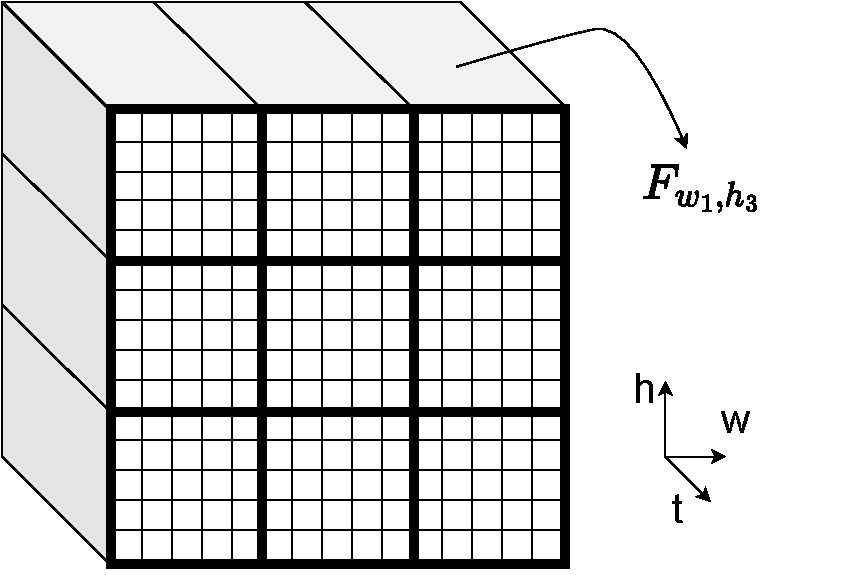
\includegraphics[width=\textwidth]{images/quantile_mapping.drawio.pdf}
        \caption{}\label{}
    \end{subcaptionblock}%
    \hspace{30mm}
    \begin{subcaptionblock}{0.20\textwidth}
        \centering
        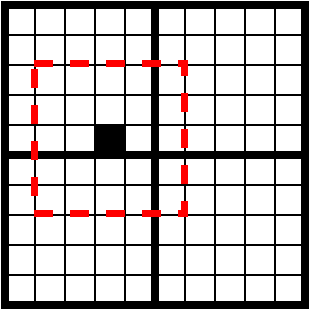
\includegraphics[width=\textwidth]{images/quantile_conv.drawio.pdf}
        \caption{}\label{}
    \end{subcaptionblock}%
    
        % \begin{subcaptionblock}{\label{cat}}
        % {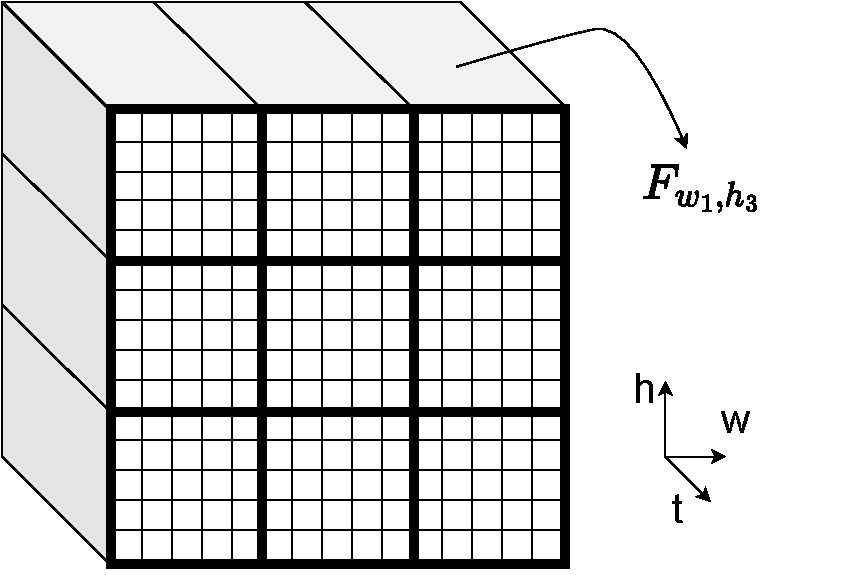
\includegraphics[width=0.5\textwidth]{images/quantile_mapping.drawio.pdf}}%
        % \subcaptionbox{\label{elephant}}
        % [0.5\textwidth]{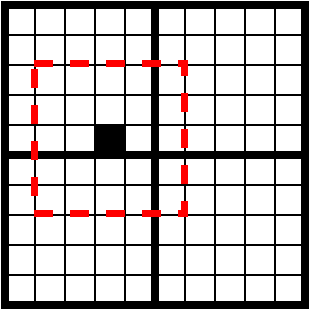
\includegraphics[width=0.25\textwidth]{images/quantile_conv.drawio.pdf}}
     % \begin{subfigure}[c]{0.48\textwidth}
     % \centering
     %     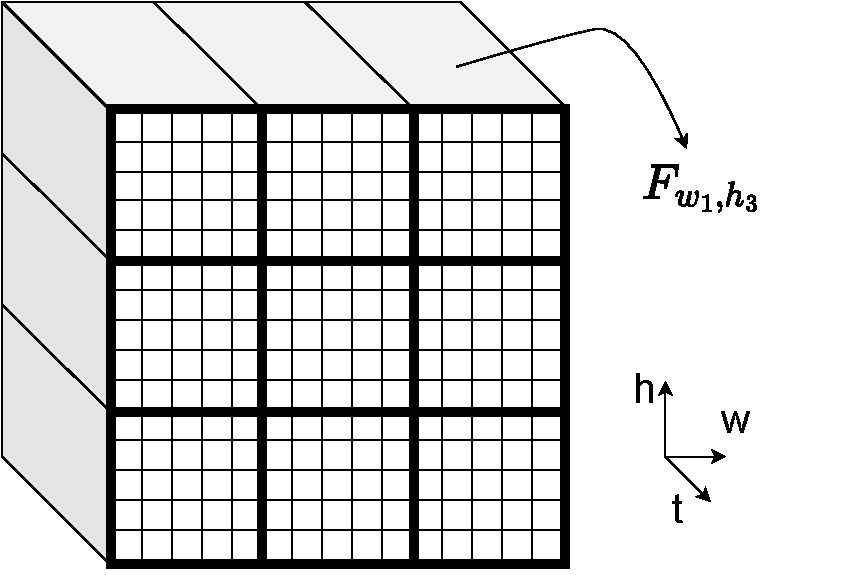
\includegraphics[width=\textwidth]{images/quantile_mapping.drawio.pdf}
     %     \caption{}
     %     \centering
     % \end{subfigure}
     % \hfill
     % \hspace{-10mm}
     % \begin{subfigure}[c]{0.25\textwidth}
     %     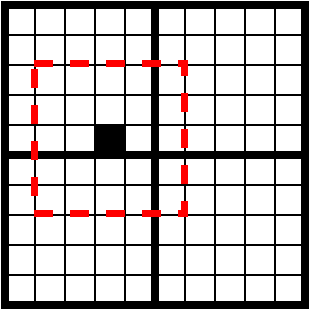
\includegraphics[width=\textwidth]{images/quantile_conv.drawio.pdf}
     %     \caption{}
     % \end{subfigure}
      \caption{a) Illustration of the general method for how grid cells are grouped together in order to estimate quantiles. In this example, the spatial domain is split into squares of $4 \times 4$ grid cells, giving 9 separate large square regions, and in each region the quantiles are calculated. b) To calculate a particular quantile for a grid point, filled in black, we perform a weighted sum of the value of this quantile calculated in the square regions nearest to that point. The weighting for each large region is proportional to the number of small squares inside the red dashed square. In this example, the red dashed square covers 25 grid cells and the weightings would be $\frac{12}{25}$, $\frac{3}{25}$, $\frac{8}{25}$, $\frac{2}{25}$.}
     \label{fig:quantiles}
\end{figure}    

From experiments we found that the typical approach of quantile mapping the GAN at each grid point individually was not a robust approach for the highest values. Therefore we aggregated the data into square regions to calculate quantiles (fig.~\ref{fig:quantiles}(a)). The intuition is that nearby points will have similar distributions and so we can gain accuracy by grouping nearby points together. 

To avoid any artefacts due to the edges of these domains, the quantiles for a given grid cell were calculated as a weighted average of the nearest squares; specifically, the quantiles used to update the values at grid cell $(m,n)$ are calculated as a weighted sum, where the weighting is calculated by drawing a square around $(m,n)$ and counting the number of grid points that fall into each quantile grouping (fig.~\ref{fig:quantiles}(b)). This is partly motivated by the ease of implementation, as this can be easily done by broadcasting the grouped quantiles to the same dimensions as the original grid, and using square convolutions with reflective padding to calculate the weighted versions of each quantiles. The length scale of the weighting window was chosen to be the same as the length scale of the quantile groupings, as this was empirically observed to produce reasonably smoothed values.

To evaluate the optimal grouping in the spatial domain, the quantile mapping approach described above was trained on the same training data as the cGAN, and then used to perform quantile mapping on forecasts in the validation set. The best parameters were chosen by calculating the quantiles over the whole domain after quantile mapping, and comparing these to the quantiles of the IMERG data over the whole domain using mean-square error. Using this method, the cGAN performed best when one set of quantiles was calculated over the whole domain, whilst the IFS forecast performed best when split into regions of size $18 \times 18$ grid points. We denote these quantile mapped models as cGAN-qm and IFS-qm.



\subsection{Assessing Sample Variability}
\label{sec:sample_var}


For many diagnostics, particularly those concerned with high rainfall events, the results can be swayed by the presence or absence of a small number of high rainfall events particular to the test year. To estimate the uncertainty due to these effects, we use bootstrapping along the time dimension~\cite{efron_bootstrap_1986}. To perform bootstrapping for a property of interest $\theta$ calculated over a set of $N$ hourly samples, we sample with replacement from these $N$ samples $M$ times, resulting in $M$ sets of samples of size $N$. Then the mean and standard error of $\theta$ can then be estimated from the mean and standard deviation of $\theta$ calculated on the bootstrap samples. Since the hours are sampled uniformly at random, this method does not take into account the correlation between adjacent hours, and so it is likely that the standard error calculated from this method is an underestimate.




\section{Evaluation on normal test set}



\subsection{Climatological properties of the forecasts}
\label{sec:climatologic}
\begin{figure}[!ht]
     \centering
     \begin{subfigure}[h]{0.45\textwidth}
         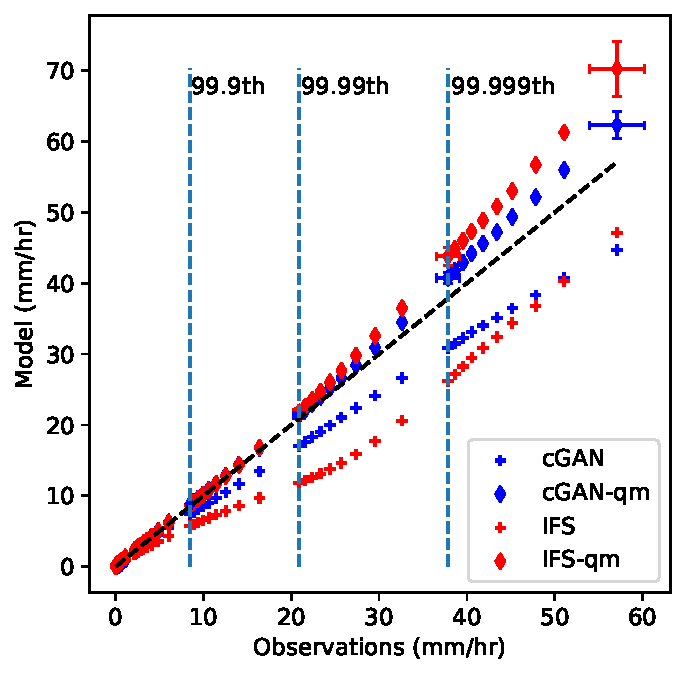
\includegraphics[width=\textwidth]{images/quantiles_total_final-nologs_217600.pdf}
         \caption{}
         \centering
     \end{subfigure}
     \hfill
     \begin{subfigure}[h]{0.5\textwidth}
         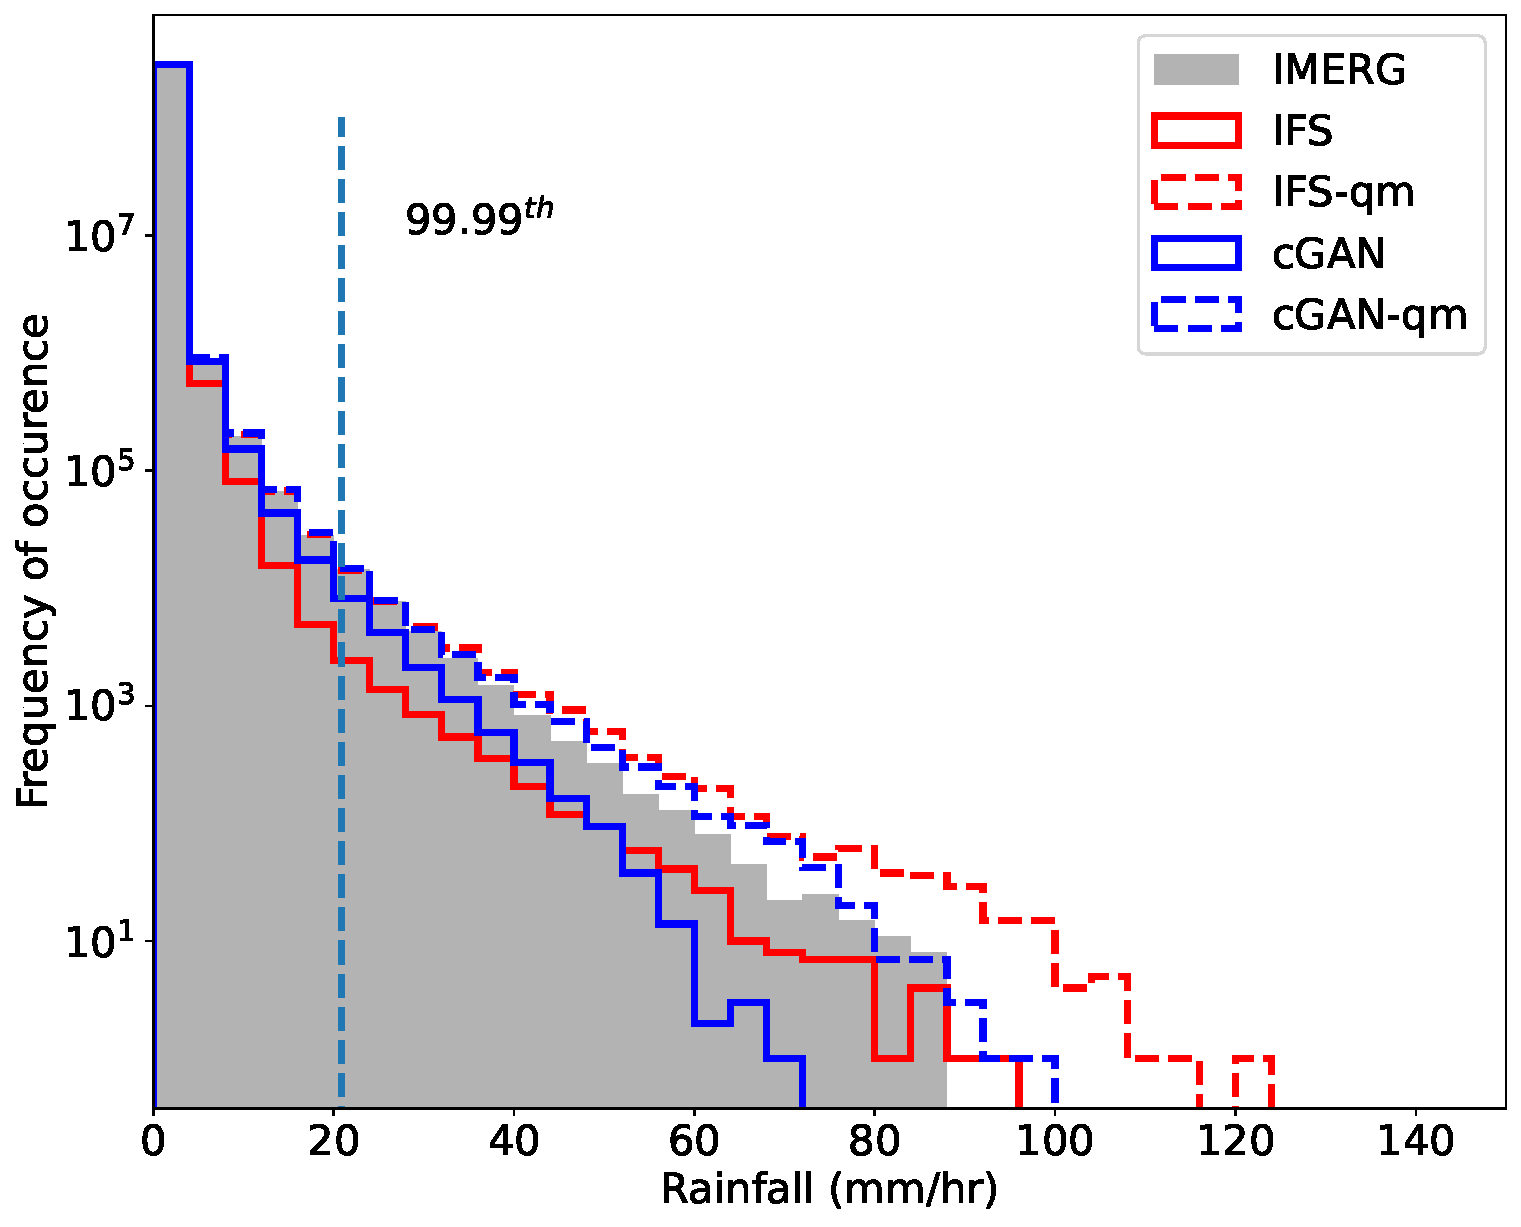
\includegraphics[width=\textwidth]{images/histograms_final-nologs_217600.pdf}
         \caption{}
        \centering
    \end{subfigure}
    \begin{subfigure}{0.48\textwidth}
     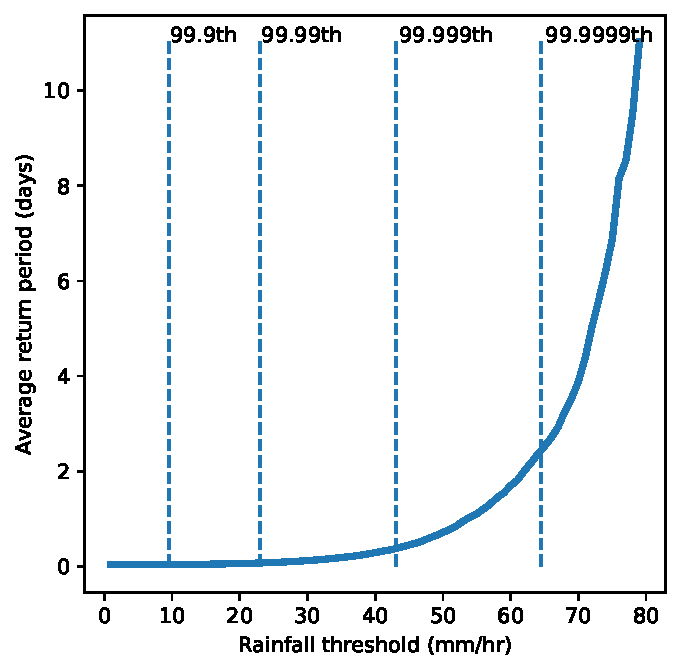
\includegraphics[width=\textwidth]{images/return_periods_train.pdf}
     \caption{}
     \end{subfigure}
     \centering
     \caption{(a) Quantile-quantile plot, up to the $99.9999^{\text{th}}$ percentile. Red circles (diamonds) indicate quantiles for the IFS (IFS-qm) model. Blue circles (diamonds) indicate quantiles for the cGAN (cGAN-qm) model. The black dashed line is the line along which a perfectly calibrated forecast would sit. The error bars indicate an estimate of 2 standard deviations from 1000 bootstrap samples b) A histogram showing the distribution of rainfall values; the vertical dashed blue line indicates the $99.99^{\text{th}}$ percentile of observed rainfall. c) The approximate return periods for different rainfall thresholds to be exceeded at any grid point in the spatial domain in the training set. The dashed lines indicate the values of particular high percentiles. }
     \label{fig:distribution}
\end{figure}

\begin{figure}[ht!]
     \centering
     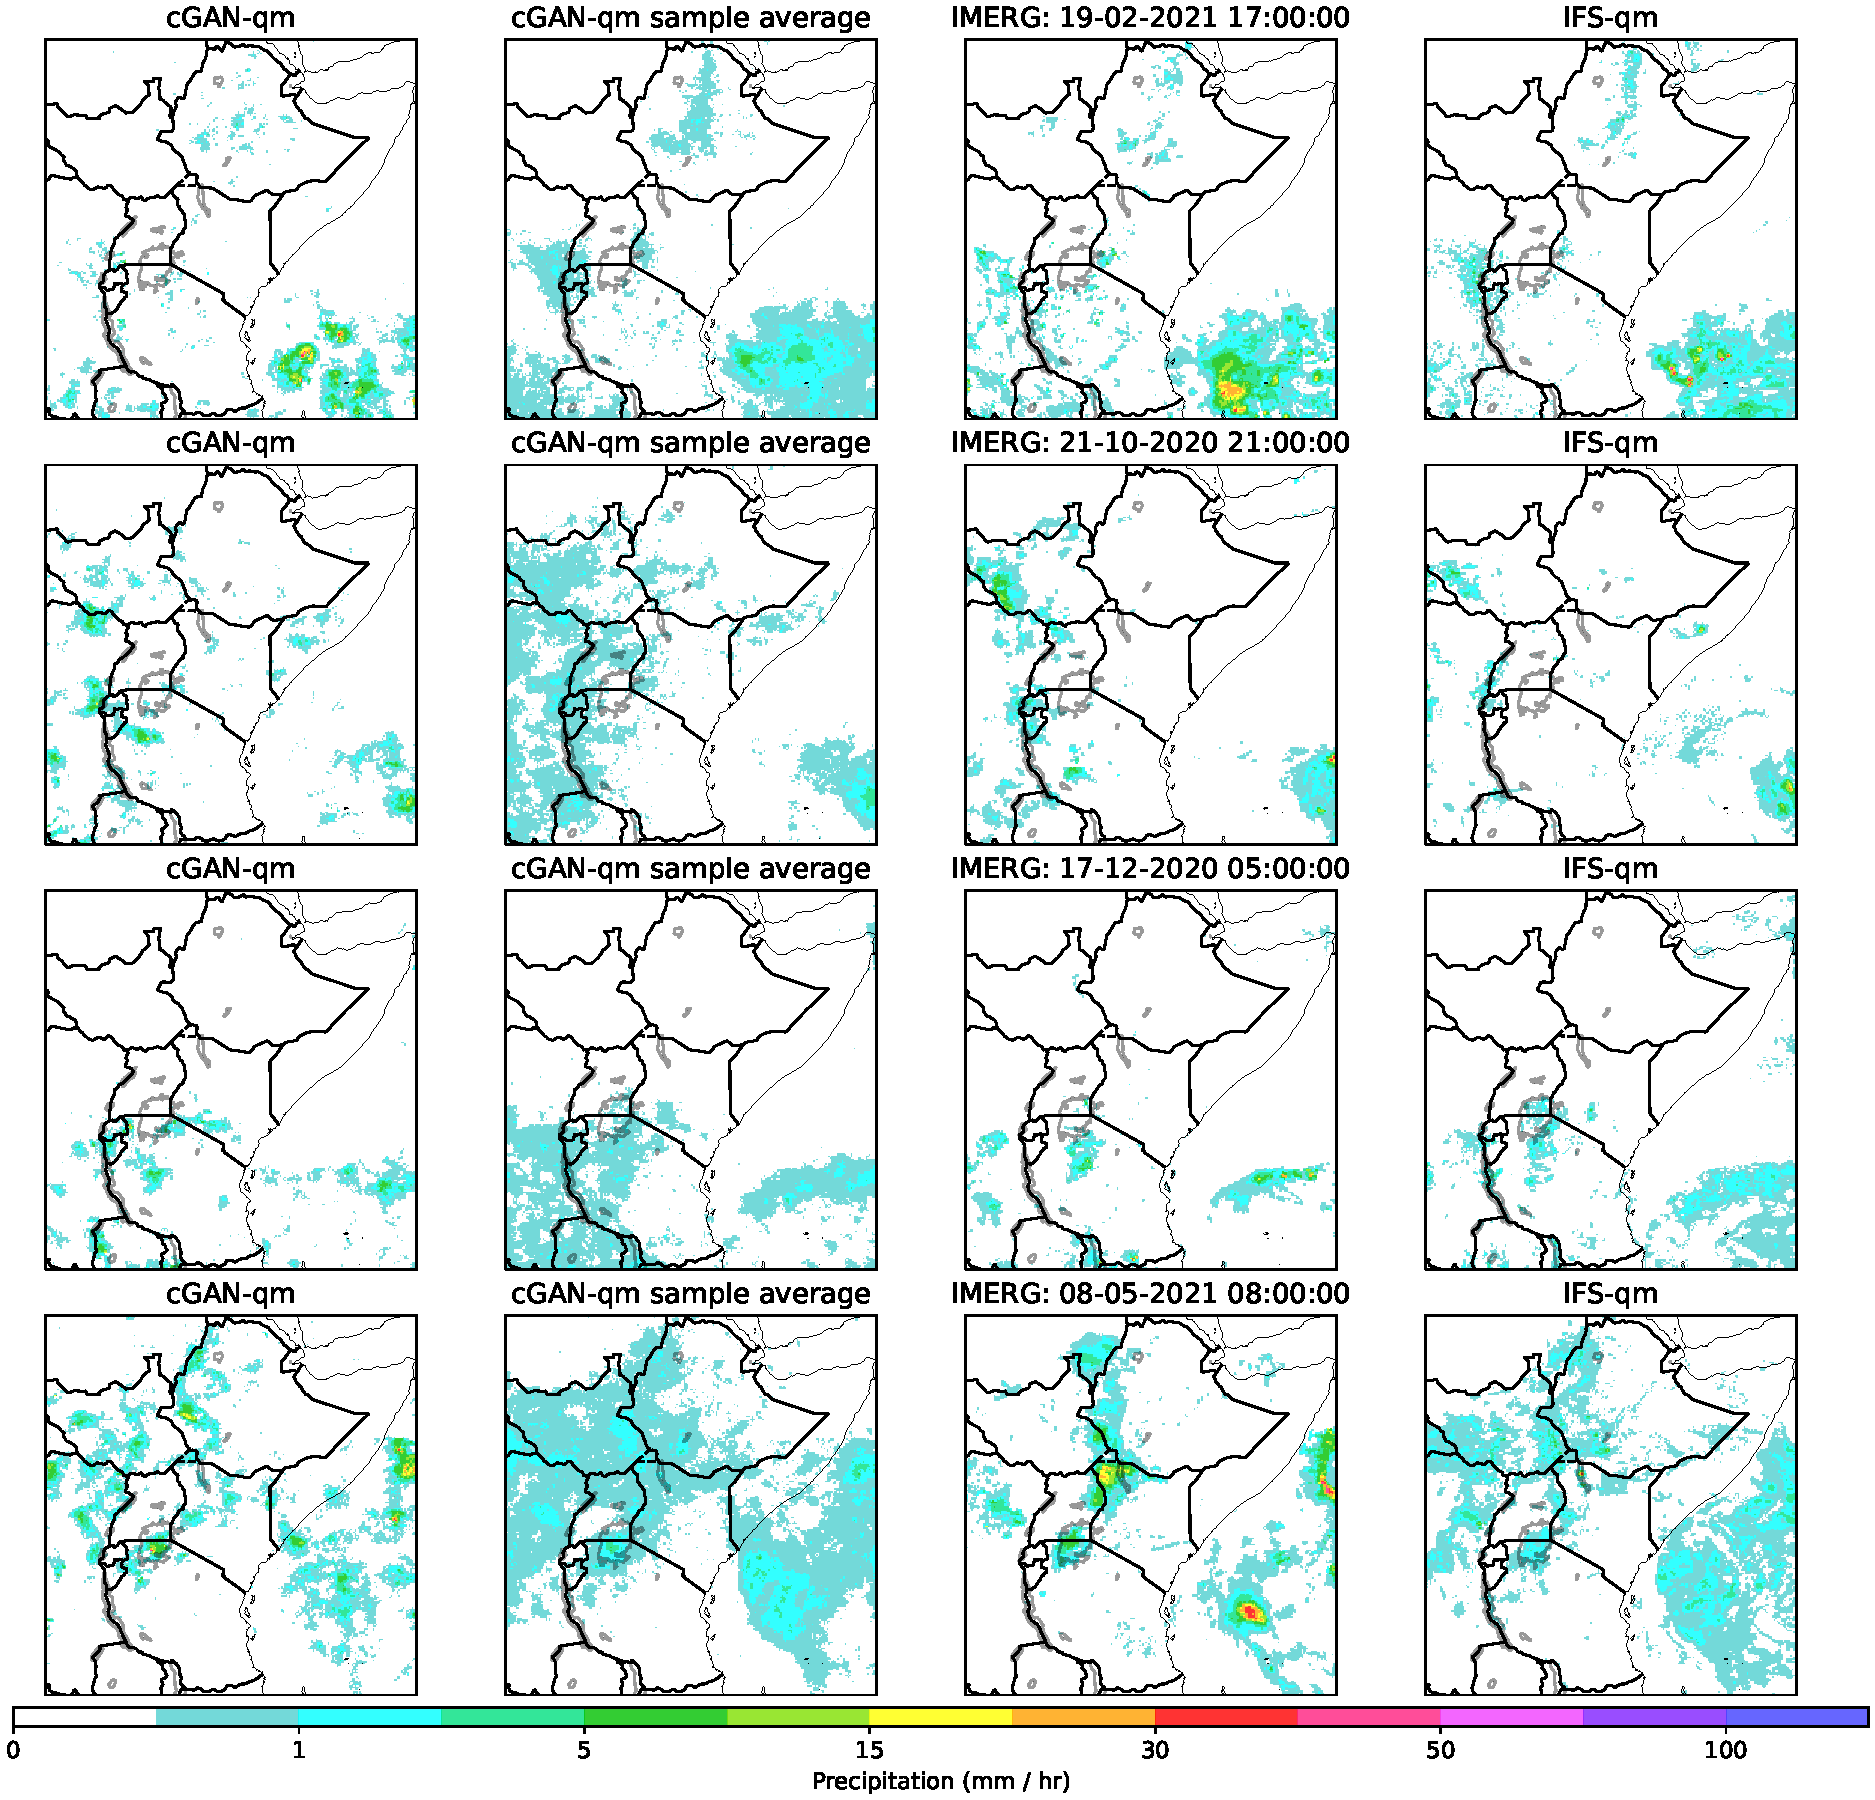
\includegraphics[width=1.05\textwidth]{images/cGAN_samples_IFS_final-nologs_217600.pdf}
     
     \caption{Example precipitation forecasts following postprocessing by the cGAN-qm model, for a selection of hours throughout the test year (first column). The columns from left to right show: a single member of the cGAN-qm ensemble, the average of 20 cGAN-qm ensemble members, the IMERG observations, the IFS-qm forecast. Each row corresponds to one time value, shown in the title of the IMERG sample. The examples were chosen from a randomly selected set of images, such that there is at least one example from each of the seasons, and also such that ...  }
     \label{fig:examples}
\end{figure}

\begin{figure}[!ht]
     \centering
     \begin{subfigure}{0.48\textwidth}
     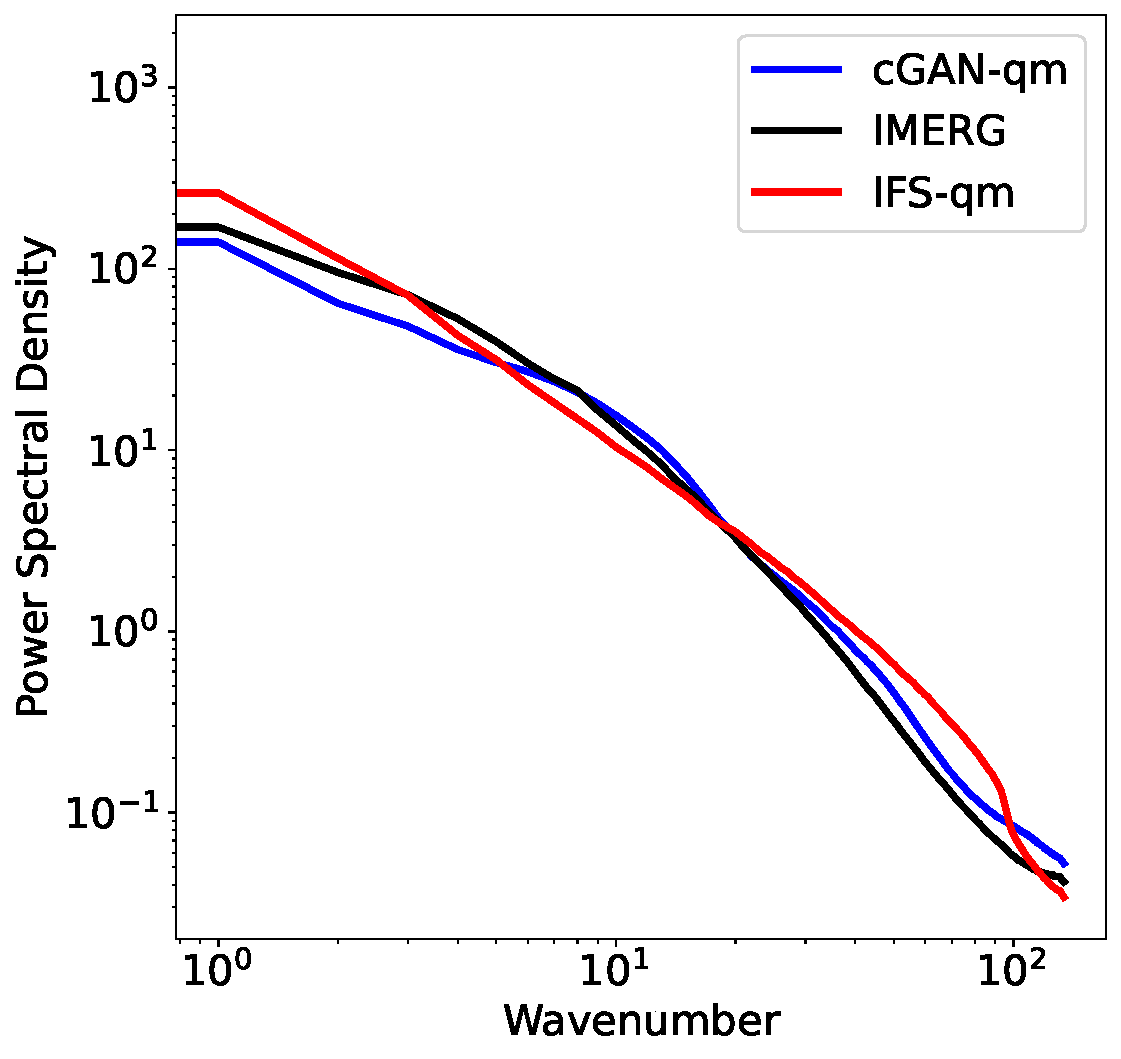
\includegraphics[width=\textwidth]{images/rapsd_final-nologs_217600.pdf}
     \caption{}
     \end{subfigure}
     
     \caption{a) Radially averaged power spectral density for the quantile mapped forecasts. The black line is for the IMERG data, the blue line for cGAN-qm, and the red line for IFS-qm. 
}
     \label{fig:rapsd}
\end{figure}











\begin{figure}[t]
    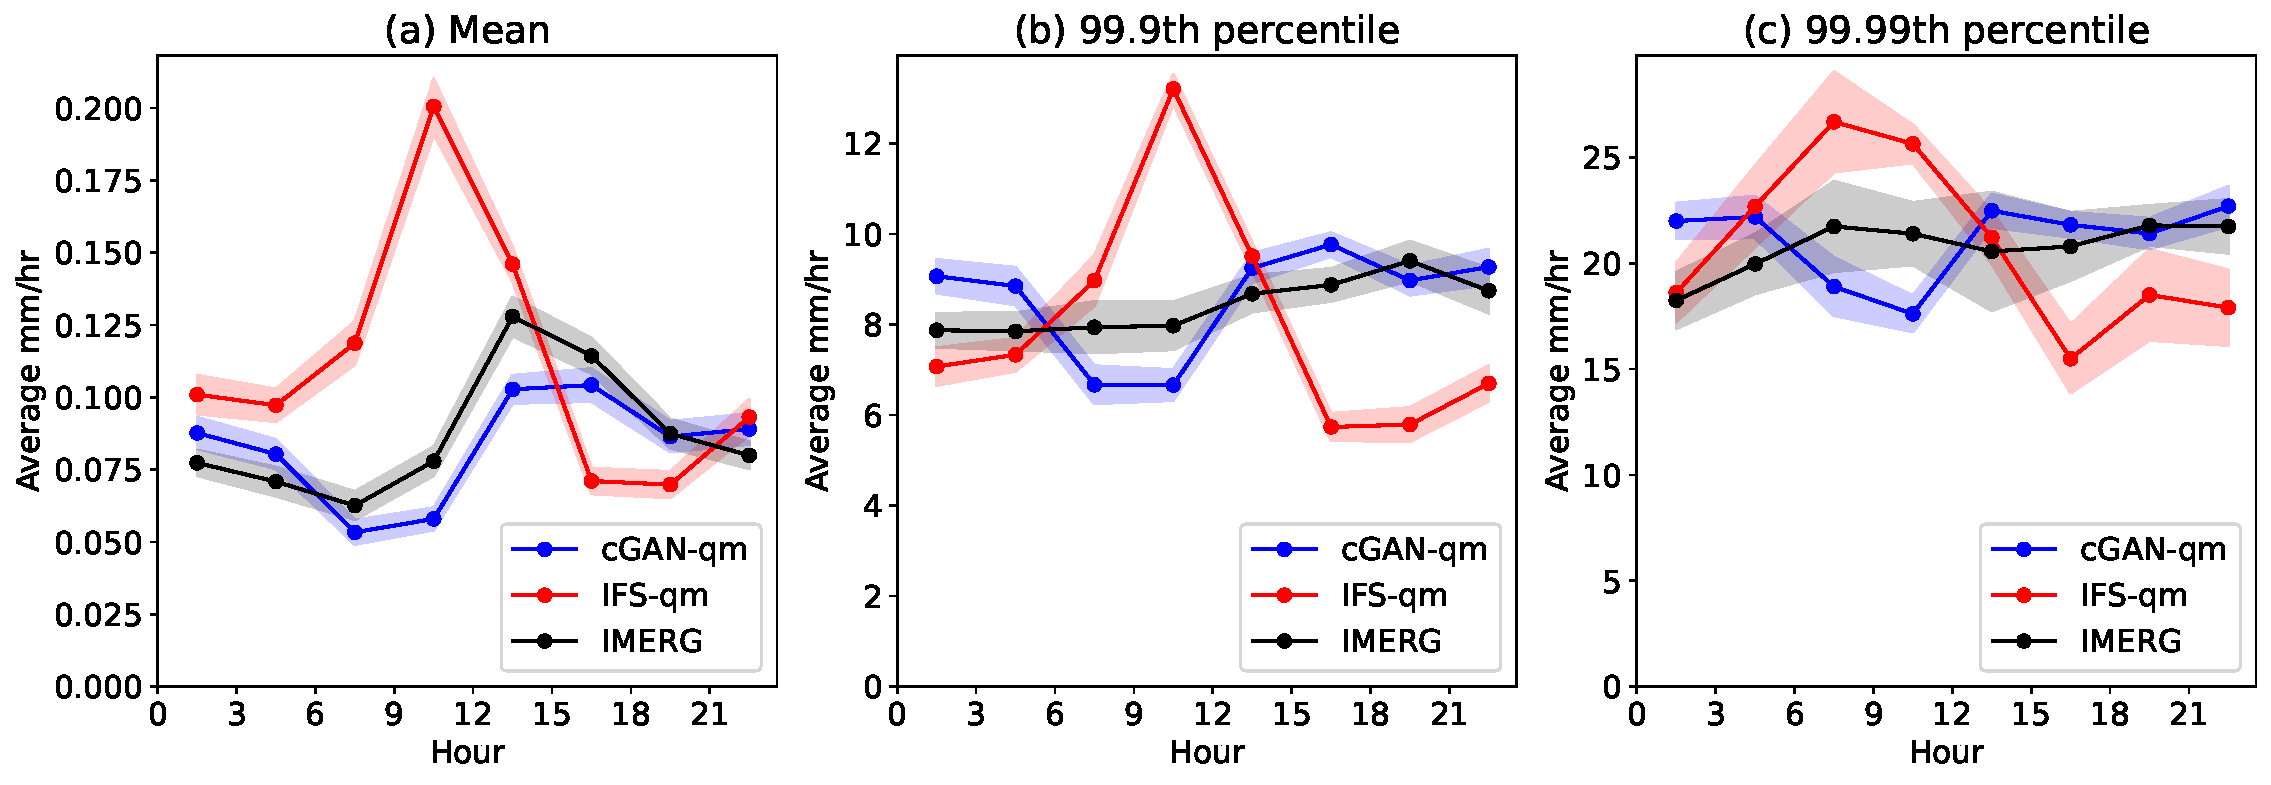
\includegraphics[width=\textwidth]{images/diurnal_cycle_final-nologs_217600.pdf}
    \centering
     \caption{Evaluation of the diurnal cycle by hour (in local time) over the whole domain in; (a) mean rainfall, (b) $99.9^{\text{th}}$ percentile, c) $99.99^{\text{th}}$ percentile, where percentiles are calculated over all individual grid points. The shaded regions indicate $\pm2$ standard errors about the mean, estimated by bootstrapping with 50 samples. Note that rainfall at the $99.9^{\text{th}}$ percentile and above is mainly concentrated over Lake Victoria and the ocean.}
     \label{fig:diurnal}
\end{figure}

\begin{figure}[t]
\centering
        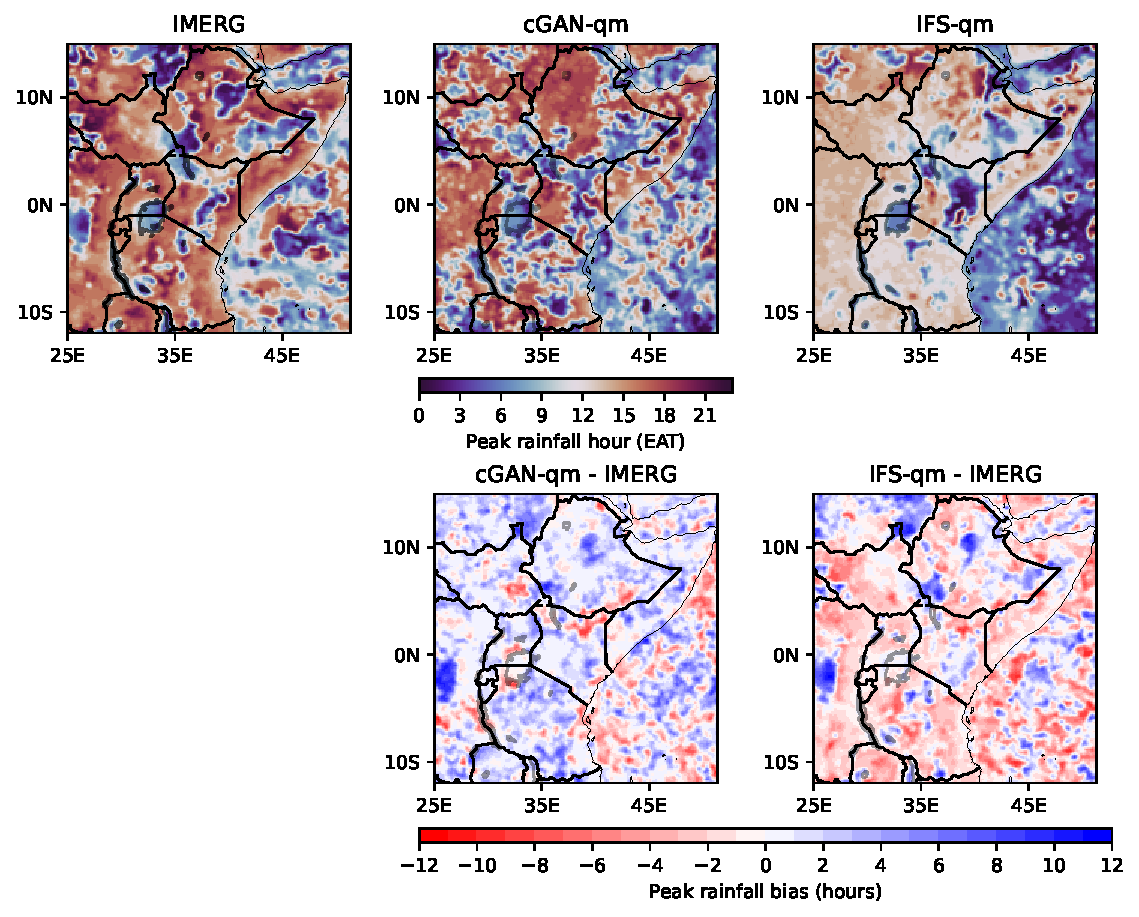
\includegraphics[width=\textwidth]{images/diurnal_cycle_map_All_final-nologs_217600.pdf}
    % \begin{subcaptionblock}{\textwidth}
    %     \centering
    %     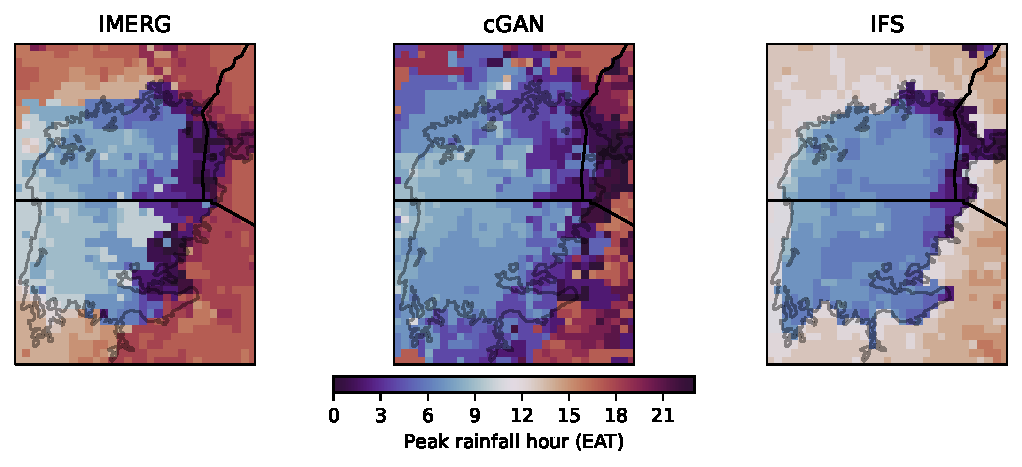
\includegraphics[width=\textwidth]{images/diurnal_cycle_map_Lake_Victoria_final-nologs_217600.pdf}
    %     \caption{}\label{}
    % \end{subcaptionblock}
     \caption{Left panel: Map of peak rainfall hour for IMERG, averaged over the whole domain. Middle panel: Difference in peak rainfall hour between cGAN-qm and IMERG. Right panel: Difference in peak rainfall hour between IFS-qm and IMERG. A 3-hour moving average along the time dimensions is applied to the data in each case before calculating the peak hour, and then spatial smoothing using a uniform filter of width 3 pixels is applied to the mapped results.}
     \label{fig:peak_hour}
\end{figure}


\begin{figure}[!ht]
    \centering
    \begin{subfigure}{0.8\textwidth}
    \centering
     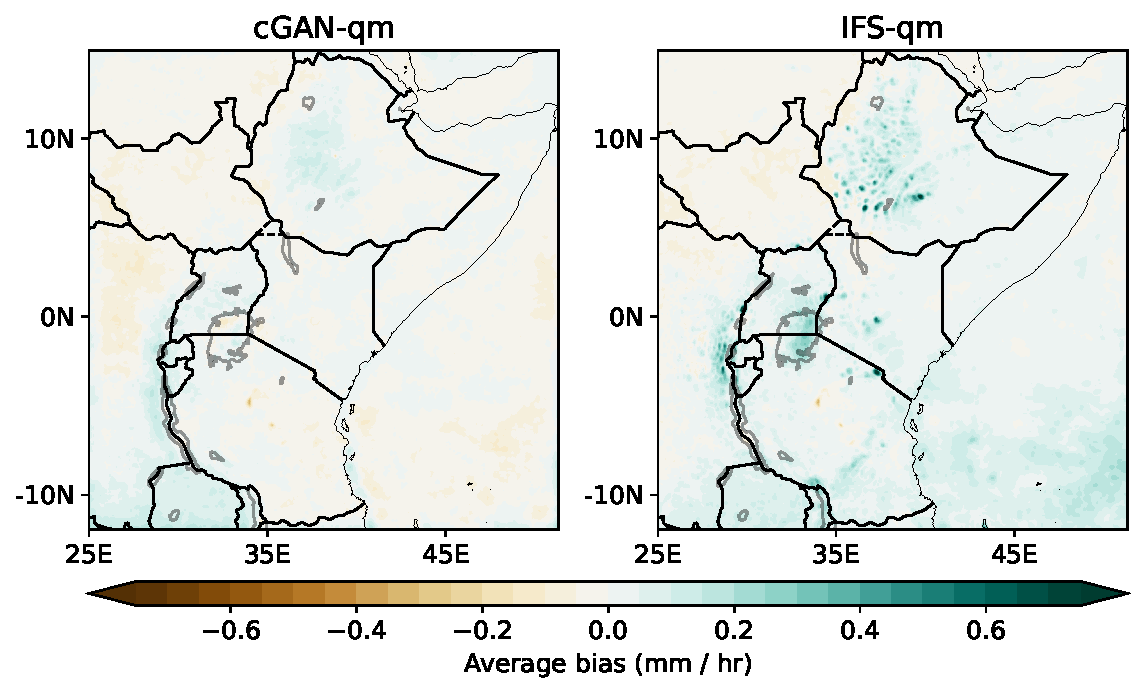
\includegraphics[width=\textwidth]{images/bias_final-nologs217600.pdf}
     \caption{}
     \end{subfigure}
     \begin{subfigure}{0.8\textwidth}
    \centering
     \includegraphics[width=\textwidth]{images/bias_std_final-nologs217600.pdf}
     \caption{}
     \end{subfigure}
    
     \caption{Biases of the cGAN-qm and IFS-qm forecasts: (a) mean bias and (b) bias in the standard deviation.}
     \label{fig:bias}
\end{figure}

\begin{figure}
\centering

    \centering
     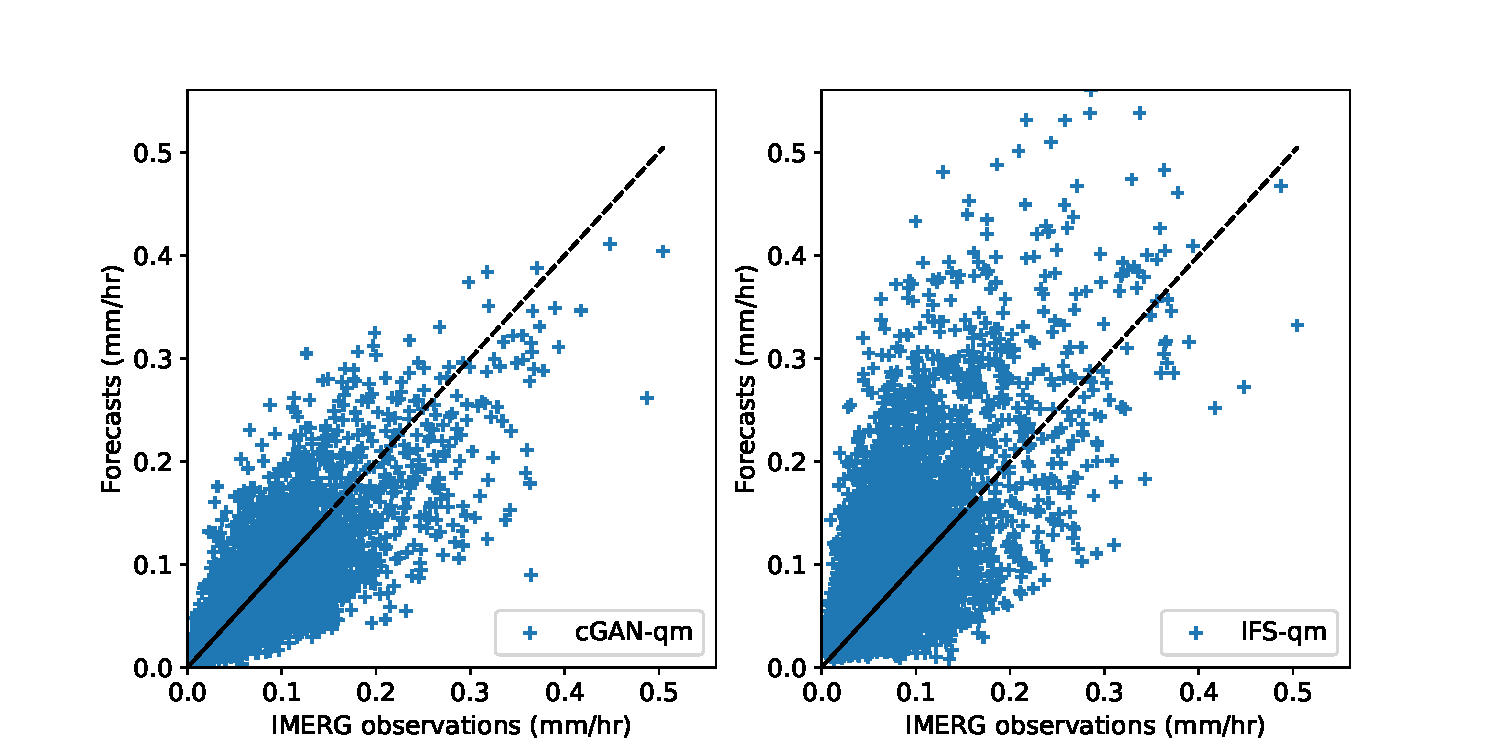
\includegraphics[width=\textwidth]{images/scatter_mean_final-nologs_217600.pdf}
     \caption{Scatter plots of predicted versus observed domain-average rainfall, for the cGAN-qm forecasts (left) and IFS-qm forecasts (right). The dashed black lines represents perfect forecasts. The Pearson correlation coefficient is 0.74 for cGAN-qm and 0.61 for IFS-qm.}
     \label{fig:bias}
\end{figure}

 We first assess how well the forecasts capture the distribution of rainfall, shown by a quantile-quantile plot and a histogram of rainfall distribution for 4000 samples, shown in Fig.~\ref{fig:distribution} (a) and (b) respectively. The raw model outputs are shown together with quantile-mapped outputs. From these we can see that the raw cGAN output is an improvement on the raw IFS output up to extremely high levels of rainfall (around 50mm/hr) beyond which point the IFS is closer to the distribution. Note that we wouldn't necessarily expect the GAN to align closely with the observed frequency distribution, since it is not explicitly trained to do so.

After both forecasts have been quantile mapped, they are much closer to the ideal line, with deviations at high quantiles which we attribute to sampling variability. The scale of sampling variability was quantified by performing 1000 iterations of bootstrapping (see Sec.~\ref{sec:sample_var}) to estimate the standard error of the quantiles. These are shown in Fig.~\ref{fig:distribution}, where each error bar shows 2 standard deviations.


In order to also get a sense of how extreme these quantile values are, we plot the approximate return period in days for a range of thresholds in Fig.~\ref{fig:distribution} (c), calculated over all hours in the test period. These are calculated as the average time gap between instances where at least one point in the domain exceeds the threshold. Note that due to correlations between hours, which artificially boost the number of times the threshold is exceeded, this will be a lower bound on the actual return period. Also note that the very high rainfall values (above around the $99.9^{\text{th}}$ percentile, $\sim20\text{mm/hr}$) are mainly concentrated over Lake Victoria and parts of the sea. 

We observed that the quantile mapped models cGAN-qm and IFS-qm performed better across the range of diagnostics considered here, and so for the remaining diagnostics in this work we will focus on these quantile-mapped forecasts.

We plot examples of the samples generated by cGAN-qm in Fig.~\ref{fig:examples}. The generated samples appear to have a realistic spatial structure, and the ensemble mean has substantial rainfall in places where rainfall is observed, indicating that at least some members include rainfall in those locations. In the bottom row example (8am on 8th May 2021) we can see cGAN-qm removing some of the excess low rainfall seen over the land and sea for the IFS-qm model. The examples on the top and bottom rows also show both models not capturing the shape and maximum intensity of the high rainfall event occurring over the sea. 

To get a quantitative picture of the spatial realism of these rainfall patterns, we plot the Radially Averaged Power Spectral Density (RAPSD) in Fig.~\ref{fig:rapsd}. cGAN-qm is closer to IMERG observations for low length scales, less than around 80km. The forecasts show opposite biases at the lowest wavenumbers, possibly due to sampling variability.

Biases in the diurnal cycle are not adjusted by the quantile mapping approach that we employ. Summary statistics of the rainfall as a function of hour are plotted in Fig.~\ref{fig:diurnal}, from which it is clear that cGAN-qm is making significant improvements to the diurnal cycle (and these are also present in cGAN). The IFS-qm forecast has a clear bias in mean rainfall around midday that is also prominent for high quantiles (Fig.~\ref{fig:diurnal} (c)), whilst the cGAN-qm mean diurnal cycle is much closer to that of observations. 

We can gain insight into which spatial locations are particularly driving this improvement from the plots of average peak rainfall hour in Fig.~\ref{fig:peak_hour}. The data is smoothed along the time axis using a centred moving average of length 3, in order to remove noise and make it easier to see any patterns in the data. The peak rainfall hour for cGAN-qm is fairly spatially noisy, but improvements can mainly be seen to occur on land. Looking at Lake Victoria (around $1^{\circ}\text{S}
$, $33^{\circ}\text{E}$), we can see that cGAN-qm correctly captures more of the nighttime maxima seen along the East coast of the lake and the morning maxima seen in the central and Western parts (see e.g.~\cite{woodhams_identifying_2019}), although it also tends to have a strong early bias in the land around the Western part of the lake.


The plot of average bias in Fig.~\ref{fig:bias} (a) shows that on average the cGAN-qm under-predicts rainfall on the test set whilst IFS-qm over-predicts. cGAN-qm also reduces the most prominent average biases of IFS-qm occurring over the Ethiopian highlands, Lake Victoria and the Western side of the East African rift, near Rwanda and Burundi. The effects on the bias in the standard deviation in Fig.~\ref{fig:bias} (b) are less obvious, there is some reduction in the sharpness of the peaks around the Ethiopian highlands, coastal regions and over the ocean, but there are also areas of increased negative bias in other parts of the ocean and in the western part of the domain over the Democratic Republic of Congo. 

The scatter plot in Fig.~\ref{fig:bias} shows how each model captures the domain-averaged rainfall; the cGAN-qm model is more tightly clustered around the ideal diagonal line, with IFS-qm more spread out and tending to over-predict. This is reflected in the Pearson correlation coefficients; 0.74 for the cGAN-qm and 0.61 for the IFS-qm. This suggests that cGAN-qm has improved the accuracy of predicting domain-average rainfall on at least some days.



\begin{figure}[t]
    \centering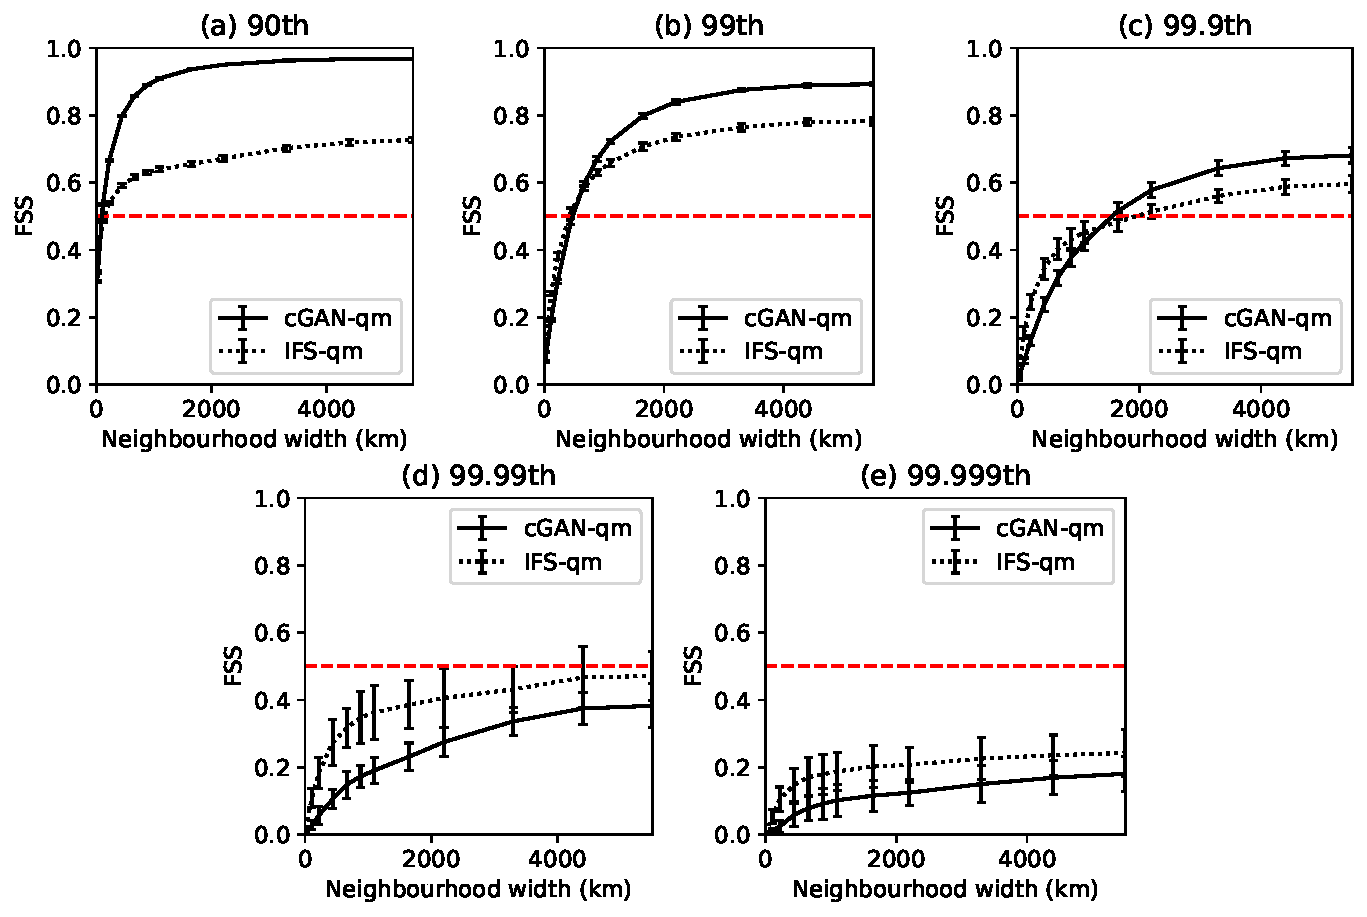
\includegraphics[width=\textwidth]{images/fss_final-nologs_217600.pdf}
     \caption{Fractions Skill Score results for different quantile thresholds (a) $90^{\text{th}}$ percentile (b) $99^{\text{th}}$ percentile (c) $99.9^{\text{th}}$ percentile (d) $99.99^{\text{th}}$ percentile (e) $99.999^{\text{th}}$ percentile. The red dashed lines indicate the `useful' threshold of 0.5 that is typically used to interpret this score. Error bars indicate $\pm2$ standard errors estimated from bootstrapping with 50 samples. Note that rainfall at the $99.9^{\text{th}}$ percentile and above is mainly concentrated over Lake Victoria and over the ocean. }
     \label{fig:fss}
\end{figure}




\subsection{Forecast skill assessment}
\label{sec:fcst_skill}

We now look at skill at predicting specific rainfall events, focusing on occurrences of rainfall above a certain threshold. We start with the Fractions Skill Score (FSS)~\citep{roberts_assessing_2008, roberts_scale-selective_2008}. In Fig.~\ref{fig:fss} we show plots of FSS for different quantile thresholds, where the quantiles are calculated over the whole domain rather than for each grid cell individually.

The value that the FSS reaches at the maximum neighbourhood size indicates the bias in the frequency with which forecasts exceed the particular rainfall threshold~\citep{roberts_assessing_2008, roberts_scale-selective_2008}, and so we can see that, up to thresholds around the $99.9^{\text{th}}$ percentile, cGAN-qm has lower overall bias. Above this threshold, whilst IFS-qm has higher FSS on average, the effects of sampling variability are significant (especially given that these error bars are likely an underestimate), and so it is unclear whether IFS-qm is performing systematically better. 

The FSS is typically interpreted relative to the `useful' criteria of $\frac{1}{2} + \frac{f_O}{2}$, and we can see that, for thresholds up to around the $99.9^{\text{th}}$ percentile cGAN-qm crosses this line at slightly lower neighbourhood size. However, it is known that skilful forecasts can lie below this line~\citep{nachamkin_applying_2015, mittermaier_long-term_2013}, and we can see that the IFS-qm achieves higher scores at lower neighbourhood sizes, which suggests improved skill at fine resolutions. 

Overall then, these results suggest that, for up to around the $99.9^{\text{th}}$ percentile cGAN-qm scores better. Above this level the sampling variability in the test set makes it hard to draw any robust conclusions, but for this test set IFS-qm shows better performance on average at the very high percentiles.



\begin{figure}[ht]
    \centering
     \begin{subfigure}[t]{0.45\textwidth}

     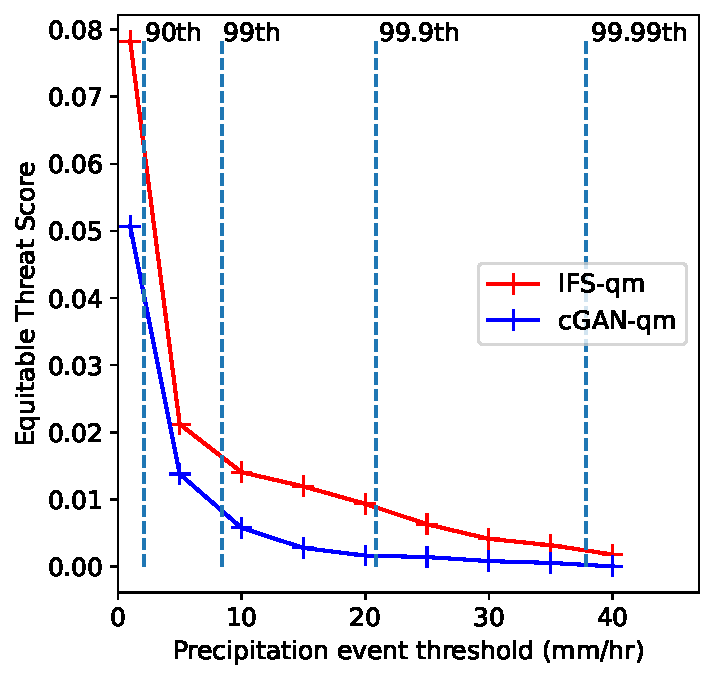
\includegraphics[width=\textwidth]{images/ets_final-nologs_217600.pdf}
     \caption{}
     \end{subfigure}
     \hfill
     \centering
     \begin{subfigure}[t]{0.49\textwidth}
     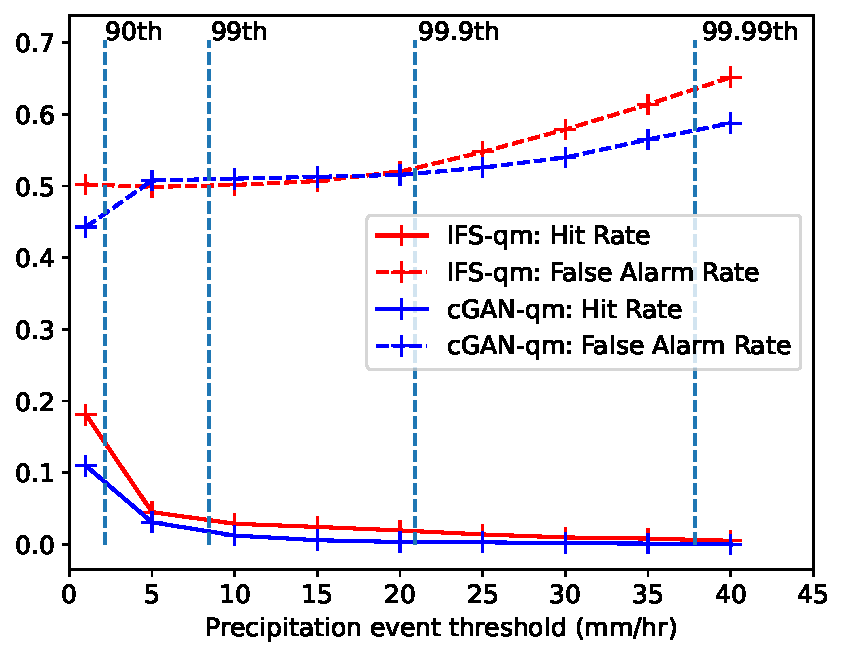
\includegraphics[width=\textwidth]{images/hit_rate_final-nologs_217600.pdf}
     \caption{}
     \end{subfigure}
     \caption{ Equitable threat score (a) and hit rate and false alarm rate (b) for IFS-qm (red) and cGAN-qm (blue) for forecasts at individual grid points, plotted against rainfall threshold. Here an event is defined as occurrence of rainfall exceeding the threshold. Note that rainfall at the $99.9^{\text{th}}$ percentile and above is mainly concentrated over Lake Victoria and over the sea.}
     \label{fig:ets}
\end{figure}


We also assess forecasts using the Equitable Threat Score (ETS)~\citep{schaefer_critical_1990, wilks_forecast_2019}, which measures the balance between the hit rate and false alarm rate, whilst accounting for the probability of random events. This score is used in operational forecast verification~\citep{mittermaier_long-term_2013} and in~\cite{manzato_behaviour_2017} was shown to be one of the most robust metrics with respect to random (unskillful) changes in the forecast.

The ETS for several thresholds over the whole domain is shown in Fig.~\ref{fig:ets} (a), for rainfall at individual grid points. This shows that IFS-qm tends to perform better by this metric, which is in agreement with the FSS results that show IFS-qm performing better at smaller length scales. In Fig~\ref{fig:ets} (b) the Hit Rate (HR) and False Alarm Rate (FAR) are shown, from which we can see that performance at low rainfall values is predominantly driven by differences in HR. For thresholds above 20mm/hr the FAR tends to increase substantially for IFS-qm, with cGAN-qm showing less of an increase.

        
\subsection{Assessment of ensemble calibration}
\label{sec:ens_calib}

\begin{figure}[!ht]
    \centering
    \begin{subfigure}[t]{0.49\textwidth}
     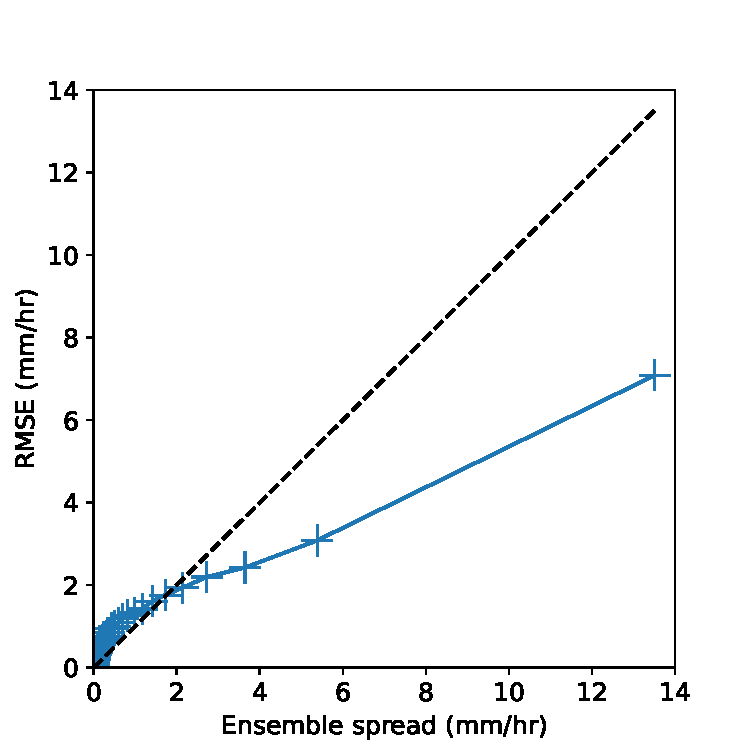
\includegraphics[width=\textwidth]{images/spread_error_final-nologs_217600.pdf}
     \caption{}
     \end{subfigure}
     \centering
    \begin{subfigure}[t]{0.49\textwidth}
     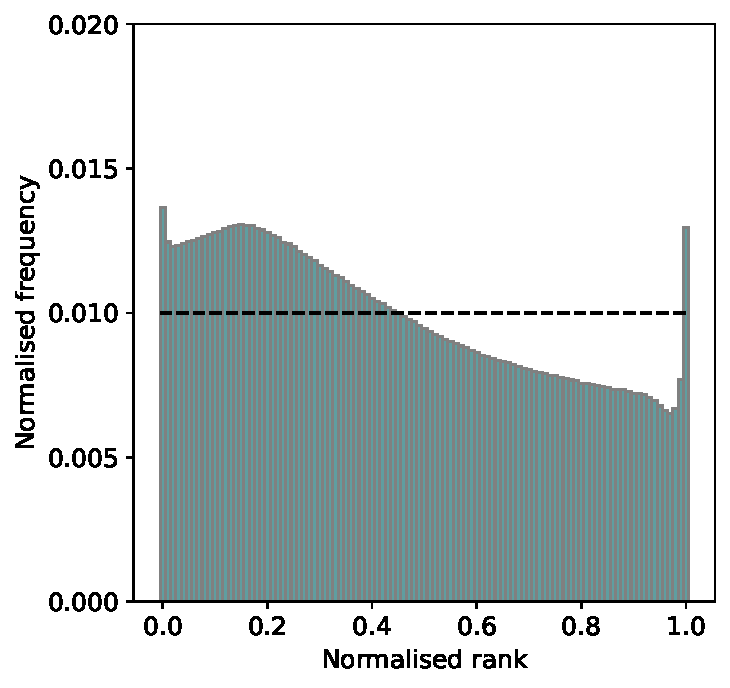
\includegraphics[width=\textwidth]{images/rank_hist_final-nologs_217600.pdf}
     \caption{}
     \end{subfigure}
     \centering
     \begin{subfigure}[t]{0.49\textwidth}
     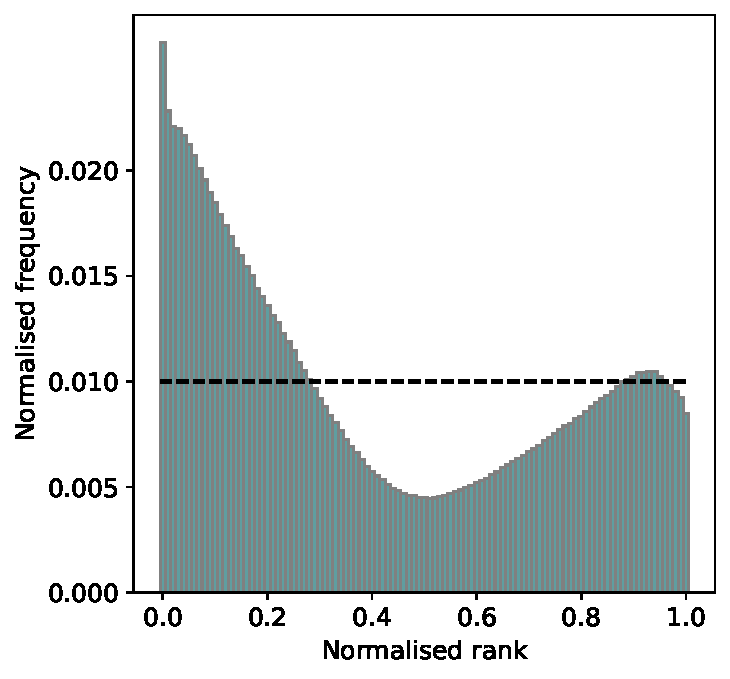
\includegraphics[width=\textwidth]{images/rank_hist_above_thr_final-nologs_217600.pdf}
     \caption{}
     \end{subfigure}
     \centering
      \begin{subfigure}[t]{0.49\textwidth}
     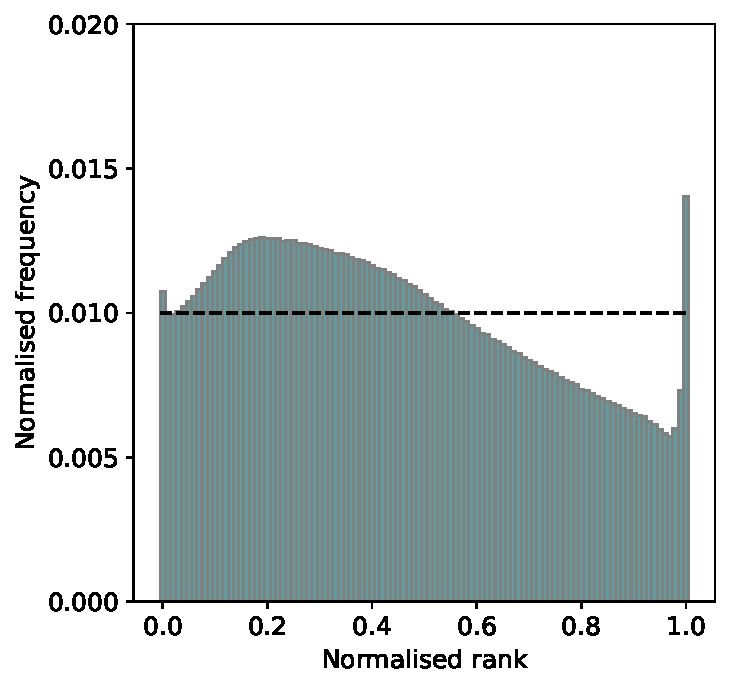
\includegraphics[width=\textwidth]{images/rank_hist_below_thr_final-nologs_217600.pdf}
     \caption{}
     \end{subfigure}
     
     
     \caption{Evaluation of the ensemble calibration of cGAN-qm, calculated using 500 samples from cGAN-qm with 100 ensemble members and evaluated at individual grid points. a) Spread error, where hourly ensemble forecasts are divided into 100 bins with different ensemble spreads. b) Rank histogram. c) Rank histogram for grid points where the cGAN-qm ensemble mean is $>0.1\text{mm/hr}$. d) Rank histogram for pixels where the cGAN-qm ensemble mean is $\leq 0.1\text{mm/hr}$. The dashed black lines represent the result for a perfectly calibrated ensemble. }
     \label{fig:ens_calib}
\end{figure}


We now focus on the probabilistic calibration of the cGAN-qm ensemble, in order to evaluate how suitable cGAN-qm samples are for use as an ensemble. Note that, there is not an ensemble NWP forecast of equivalent resolution covering the test period to compare with. These results are assessed on 500 samples drawn randomly from the test year, each with 100 ensemble members. 

Conceptually, the probabilistic skill depends on variability of both the deterministic and stochastic components of the forecasts. The deterministic component of cGAN-qm is identified with the population ensemble mean and the stochastic component with the distribution of individual members about the mean.

In Fig.~\ref{fig:ens_calib} (c) we show the spread error diagnostic~\citep{leutbecher_ensemble_2008}, where the forecasts are binned into 100 different intervals of the forecast ``spread'', which equals the standard deviation. This specifically tests the calibration of the stochastic component of the predictions alone, which has not been examined in previous studies of ML-based forecasts, and it is of interest how well a GAN can learn to represent this. For a perfect forecast, the spread of the ensemble will equal the ...

From the figure we can see that that the spreads of forecasts from the cGAN-qm ensemble cover a substantial range and are closely correlated with the RMSE, showing that cGAN-qm skilfully distinguishes between situations with higher and lower predictability. The ensemble tends to be under-dispersed (i.e.~over-confident) in relatively predictable situations (low ensemble spread), and over-dispersed (i.e.~under-confident) in relatively less predictable situations (high ensemble spread). Whilst the ensemble isn't calibrated perfectly, it is also reassuring to see that cGAN-qm has not fallen into the common failure mode of predominantly producing predictions close to the most likely result, which would produce forecasts with far too low ensemble spread.

Fig.~\ref{fig:ens_calib}(b) shows a rank histogram~\citep{wilks_forecast_2019} of forecasts for rainfall at individual grid points. This depends on both the deterministic and stochastic components of the predictions. The ensemble deviates from being perfectly calibrated, and appears to be made up of a mixture of behaviours. In general it is hard to uniquely attribute forecast behaviour from a rank histogram~\citep{hamill_interpretation_2001}: a U-shaped distribution can be indicative of under-dispersion of the ensemble, but can also be a mixture of over- and under-forecasting biases. 

In order to shed light on this, we also calculate rank histograms conditioned on whether the cGAN-qm ensemble mean indicates relatively wet or dry weather. We condition on the mean because its sampling variability is lower, and so using this as the conditioning variable greatly reduces the selection bias that would occur if we conditioned on the observed rainfall. In Fig.~\ref{fig:ens_calib} (c) and (d) we show rank histograms conditioned on the cGAN-qm ensemble mean being $>0.1\text{mm/hr}$ and $\leq 0.1\text{mm/hr}$, respectively. In Fig.~\ref{fig:ens_calib} (c) we can see a clear U-shape for the wet hours, indicating under-dispersion, and a tendency to predict higher than the observations. From Fig.~\ref{fig:ens_calib} (d) we can see that the dominant behaviour at low rainfall intensity is over-prediction and over-dispersion. 

TODO: explain spread erro plot in light of rank histogram?

% There is also an apparent contradiction between the spread-error plot result and the rank histogram: The spread-error plot appears to show over-dispersion with high rainfall values, while the rank histogram appears to show under-dispersion at high rainfall values. An explanation for this could be down to the fact that the rank histogram measures ordering and is insensitive to the particular error values, unlike the spread-error. Then potentially the spread-error is being skewed by a small number of forecasts that produce very high predictions, which doesn't show up on the rank histograms.

\section{Evaluation on extreme test set}

In this section we evaluate the performance of the cGAN-qm model on the extreme test set, March-May 2018.


\begin{figure}[h]
     \centering
     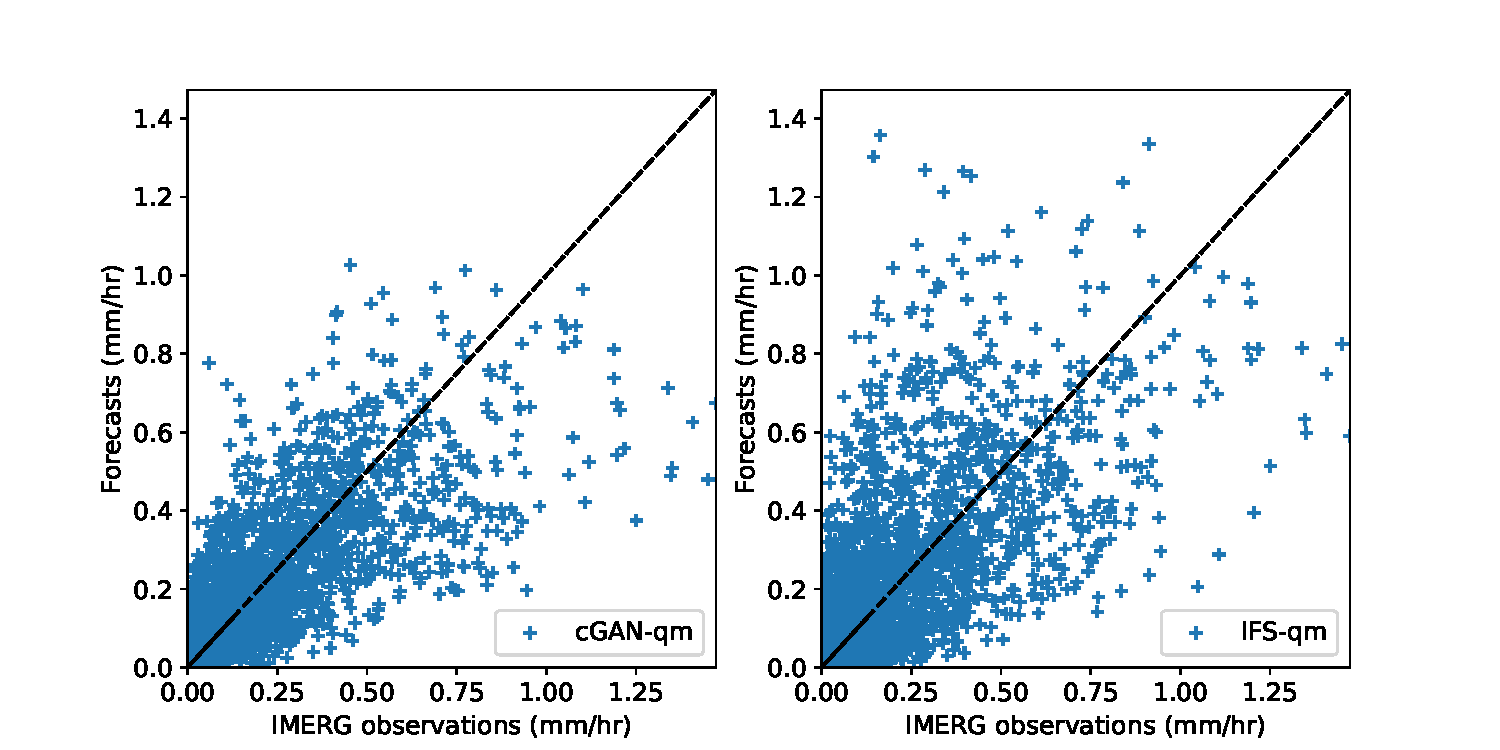
\includegraphics[width=1.05\textwidth]{images/scatter_cl100-medium-nologs_217600_kenya.pdf}
     
     \caption{
     }
     \label{fig:examples}
\end{figure}

\begin{figure}[ht!]
     \centering
     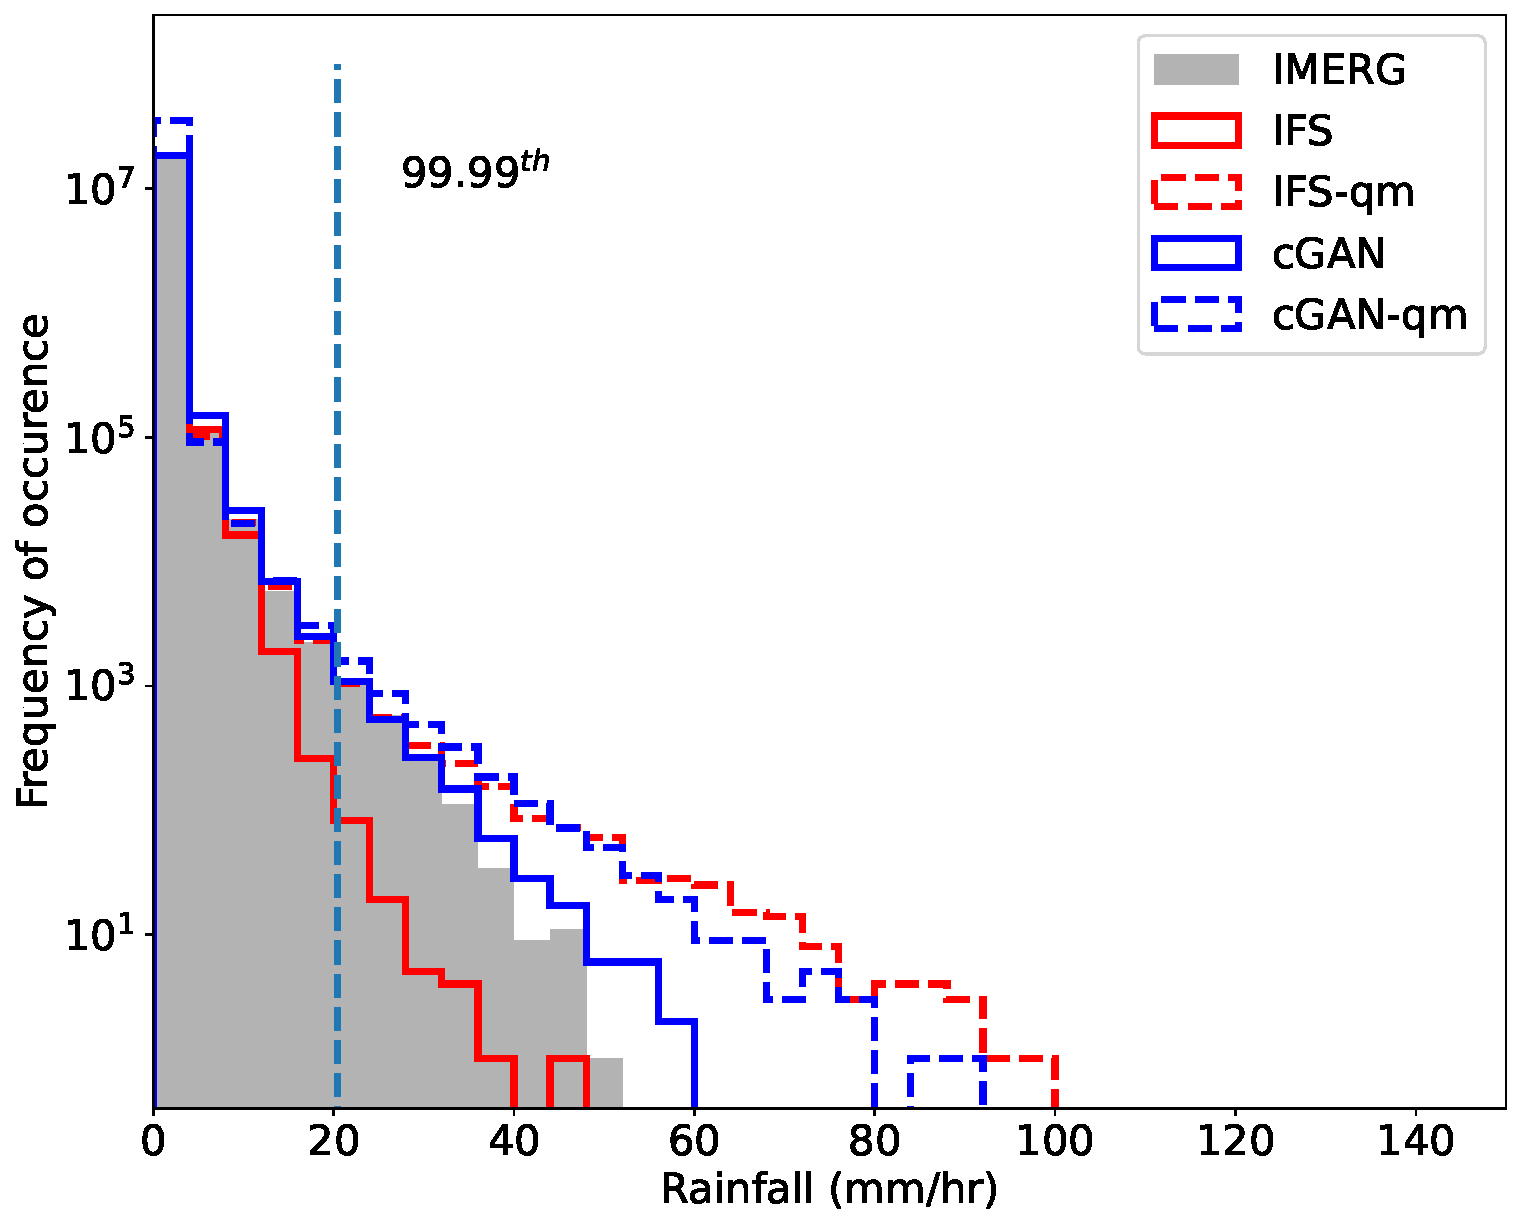
\includegraphics[width=0.5\textwidth]{images/histograms_final-nologs-mam2018_217600_kenya.pdf}
     
     \caption{
     }
     \label{fig:examples}
\end{figure}

% A visual inspection of samples produced by the cGAN (Fig.~\ref{fig:cgan_sample}) confirms that it produces realistic spatial rainfall patterns; general features seem to be that the cGAN removes some of the wet bias at low intensities, and more accurately represent the high intensity rainfall. We use the radially-averaged spectral density as a measure of the spatial structure of the forecasts, shown in Fig.~\ref{fig:metrics}(a); this shows that the cGAN samples have a closer resemblance to the spectral density than the original forecast (although the cGAN tends to overpredict at high wavenumber - corresponding to smaller length scales). Compared to the quantile mapped forecast, the cGAN appears to do better at medium-range wavenumbers, but less well at higher wavenumbers. The cGAN also successfully corrects the position of the peak in diurnal cycle of the IFS (shown for the whole region in Fig.~\ref{fig:metrics}(c)), although it shows an overprediction in the peak height.

% Quantile-quantile plots reveal that the cGAN is able to correct the forecast bias up to the 99.99th percentile. However, beyond this there is extreme overprediction of high rainfall; this is an effect noted in~\citep{harris_generative_2022}, for which they introduced a rainfall threshold to cut off extremely high values. Also all the scores in~\citep{leinonen_stochastic_2020} were calculated after converting the rainfall to the range [0,1], and so any errors in intensity would not have registered in their analysis. A natural question to ask is why the discriminator in the GAN is unable to pick up on these extreme intensities; one explanation could be that GAN discriminators are known to be poor at learning for any frequency components in the image that have low magnitude (which in this case are the high frequency components)~\citep{schwarz_frequency_2021}. 

% note that the results capture the earlier peak rainfall in southeastern Lake Victoria, as mentioned in \citep{finney_implications_2019}.

\section{Conclusions}


In this work we have investigated the use of a conditional Generative Adversarial Network to postprocess the ECMWF IFS HRES forecast over equatorial East Africa and to generate an ensemble forecast. Quantile mapping was applied to the IFS forecast (labelled ``IFS-qm'') to provide a strong baseline, and also to the cGAN output (labelled ``cGAN-qm'') in order to combine the strengths of both conventional postprocessing methods and machine learning.

The cGAN-qm and IFS-qm rainfall frequency distributions are comparable, with both models tending to over-predict at high rainfall values (more than around 20mm/hr) on the test dataset. Quantile mapping perfectly corrects the distributions in the training data, so this indicates the magnitude of sampling variability in the training and test sets. The cGAN-qm removes some of the biases in the IFS-qm model, as demonstrated by plots of the average bias and a scatter plot of domain averaged rainfall.

cGAN-qm postprocessing substantially improved the diurnal cycle, which is known to be particularly problematic for conventional NWP models to capture. The cGAN-qm model demonstrated a substantial improvement in the average diurnal cycle over the whole domain, which persisted when looking at the diurnal cycle of high quantiles. However, there is substantial spatial noise in the cGAN-qm peak rainfall hour. Using time as an input variable may be one way to improve the learnt relationships.

To assess the ability of the model to predict events at a range of spatial scales, the Fractions Skill Score (FSS) was used. Up to a high percentile ($99.9^{\text{th}}$) the cGAN-qm shows generally higher FSS scores, particularly at larger neighbourhood sizes, demonstrating that the cGAN-qm has lower bias in the frequency of pixels exceeding the threshold. For extremely high rainfall values, the IFS-qm forecast had a higher score, though when sampling variability is taken into account this difference is not significant. To evaluate the ability of each forecast to predict rainfall events at individual points and times, without accounting for spatial structure, the Equitable Threat Score (ETS) was used; the IFS-qm model achieved higher ETS at all thresholds, although the scores were nevertheless quite low.



The calibration of the cGAN-qm ensemble was assessed via a spread-error plot and rank histograms. Both diagnostics indicate a mixture of under-dispersion and over-dispersion across different rainfall events. From conditioning of the rank histograms on the magnitude of the ensemble mean prediction, the behaviour appears to be under-dispersion in rainy hours and over-dispersion at lower rainfall values.

Overall, these results highlight the subtlety in identifying the improvements a cGAN can bring. Whilst the cGAN can significantly improve the raw IFS forecast, the improvements can be more subtle when compared with a strong existing postprocessing method like quantile mapping. Compared to the quantile mapping baseline, the improvements are mainly in the diurnal cycle and the scores for rainfall events at low to medium rainfall intensities. One limitation we have in this work is the lack of a baseline ensemble to compare probabilistic forecasts against; towards the end of this project, the ECMWF IFS released ensemble forecast data at the same resolution, so going forward it would be ideal to compare our ensemble predictions to these. 
 
In general, forecast postprocessing and verification is more meaningful when done towards a particular forecast user's needs, as this allows informed decisions to be made as to how to improve the model. So in future work it would be best to target a particular use-case for these forecasts, and this would also inform the best way to train the generative model. Since the focus of this work is on short term forecasting, which could aid with applications such as flood warnings, it would be insightful to evaluate whether using the cGAN-qm predictions improves flood forecasts. Over Lake Victoria, one of the main hazards is high winds, and whilst rainfall can serve as a proxy for when these winds may happen, it would be interesting to see how the cGAN would perform at postprocessing wind speeds as well, perhaps with multivariate output. It is also important to evaluate forecasting systems such as this on extreme events (Watson, 2022). We have held back a part of the data (the 2018 long rains) for a potential future evaluation.

We have trained and evaluated on the entire domain as a whole, but since the domain behaviour is very heterogeneous it could be better to train and/or evaluate the models over smaller areas of more importance, such as river basins prone to flooding, areas managed by a particular disaster relief agency, areas grouped by climatological similarity, or areas where impacts are particularly high (e.g.~high population density areas). Given the significant effect of Lake Victoria on the local climate, a separate lake and sea mask may also be effective in improving forecasts in that area, and it may be better to train a separate model over that region.


% There are many possible standard machine learning methods that would be good to try, such as spectral normalisation or batch normalisation after the convolutions as used in~\cite{ravuri_skilful_2021}, or a more nuanced scheme to weight the rainier days more heavily, which given the particularly dry climate seen here may well make significant improvements if performed properly. There are also additional terms we could use in the loss function, such as RAPSD, pooled spatial values, or Fractions Skill Score, that we may expect to help produce well-calibrated forecasts.

There may also be additional variables that are not currently fed into the model that could be useful. For example, location-specific parameters such as latitude or longitude, or an embedding of location as done in~\cite{rasp_neural_2018}. There is potential that these would improve the results by learning behaviours that are specific to a region and that only weakly depend on the input variables we have. Also we implicitly assume that the IFS forecast captures all of the useful information about phenomena such as the Indian Ocean Dipole, Madden-Julian oscillations and ENSO, which are known to be important factors for forecasting extreme rainfall~\citep{wainwright_extreme_2021, palmer_drivers_2023}. It would be insightful to use indexes of these drivers as additional input, and/or sea surface temperatures in relevant parts of the Indian Ocean. It would be interesting as well to include the initial state of the forecast, if available, to see whether the machine learning model is able to correct for errors in how the IFS evolves this initial state, or storm activity from the previous day, which has been shown to be useful in predicting morning storm activity~\citep{thiery_early_2017}. 

There are also other promising machine learning models that would be interesting to compare with, to see if performance improvements can be made. Particularly promising approaches would be diffusion models~\citep{addison_machine_2022, leinonen_latent_2023}, since they appear to perform well and are easier to train, and models trained directly on a suitable loss function such as the energy score.

\section*{Acknowledgments}

Funding etc

Bristol uni cluster.

\bibliography{references_z}

\appendix

\section{Forecast variables used}\label{app:fcst_vars}
The IFS variables used to train the model are shown in Table~\ref{tab:vars}, definitions taken from~\citep{ecmwf_parameter_2023}.

The preprocessing methods mentioned in the table are as follows, using the year 2017 as the reference period:
\begin{itemize}
    \item Minmax: calculate the minimum $d_{\text{min}}$ and maximum $d_{\text{max}}$ over the reference period, and then transform each value $v$ according to $(v - d_{\text{min}}) / (d_{\text{max}} - d_{\text{min}})$.
    \item Max: calculate the and maximum $d_{\text{max}}$ over the reference period, and then transform each value $v$ according to $v  / d_{\text{max}}$.
    \item Log: Transform each value $v$ according to $\log_{10}(1+v)$.
\end{itemize}
\begin{table}[ht!]
\centering
\begin{tabular}{c | c | c } 
 \hline
 Variable name & Symbol & Pre-processing applied \\ [0.5ex] 
 \hline\hline
 2 metre temperature &2t & Minmax  \\
 Convective available potential energy &cape & Log \\
 Convective inhibition &cin & Max \\
Convective precipitation &cp & Log \\
Surface pressure & sp & Minmax  \\
Total column cloud liquid water &tclw & Max \\
Total column vertically-integrated water vapour&tcwv & Log \\
Top of atmosphere incident solar radiation&tisr & Max \\
Total precipitation &tp & Log \\
Relative humidity at 200hPa  &r200 & Max \\
Relative humidity at 700hPa  &r700 & Max \\
Relative humidity at 950hPa  &r950 & Max \\
Temperature at 200hPa &t200 & Minmax \\
Temperature at 700hPa  &t700 & Minmax \\
Eastward component of wind at 200hPa &u200 & Max \\
Eastward component of wind at 700hPa &u700 & Max \\
Northward component of wind at 200hPa&v200 & Max \\
Northward component of wind at 700hPa &v700 & Max \\
Vertical velocity at 200hPa &w200 & Max \\
Vertical velocity at 500hPa &w500 & Max \\
Vertical velocity at 700hPa &w700 & Max \\
 \hline
\end{tabular}

\caption{IFS variables used to train the model, as well as the normalisation applied to each variable. See text for description of the different preprocessing types.}
\label{tab:vars}
\end{table}


\end{document}
